\documentclass{article}
\usepackage{graphicx} % Required for inserting images
\usepackage{listings}
\usepackage{makecell}
\usepackage{amsmath}% http://ctan.org/pkg/amsmath
\usepackage{float}
\usepackage{tablefootnote}
\renewcommand\theadalign{cl}
\usepackage{iclr2024_conference,times}
\usepackage{hyperref}
\usepackage{url}


\title{Inductive Transformers: How Language Models Form Concepts, And How to Make Them Even Better At It}
\author{Ben Vigoda\thanks{Direct correspondence to ben@benvigoda.com.}\hspace{0.5em},  Thomas Rochais}

\date{September 2023}
% \iclrfinalcopy % Uncomment for camera-ready version, but NOT for submission.

\begin{document}

\maketitle

%\tableofcontents

\begin{abstract}
We present a new approach to designing additional inductive bias into transformers to enable tighter conceptual organization, greater conceptual control, and higher levels of conceptual abstraction. This is a paper for those who would like to understand why transformers are structured the way they are and how new versions could be designed for ``neuro-diversity'' -- to learn differently from the same data.  This family of inductive bias requires only modest modifications to transformer activation functions. We explain the approach and give an illustrative example simulation.
\end{abstract}

% \tableofcontents

\section{Introduction and Prior Art}

Our goal is to create language models that learn better organized concepts, more controllable concepts~\citep{wang2023easyedit, meng2023massediting, hernandez2023inspecting}, and more abstract concepts. This could in turn help unlock a range of enhanced abilities including better causal reasoning, iterative experimentation, longer range planning, longer chains of reasoning, curiosity, and introspection.

Causal reasoning requires the ability to intervene between connected concepts in a model~\citep{pearl1995causal}. Iterative experimental design and interpreting results requires the ability to structure latent concepts to create hypotheses and explain observed data~\citep{lu2022unified}.  Long-range plans and chains of reasoning require the ability to compose sequences of latent concepts~\citep{lake2017building, oh2017zero, shinn2023reflexion}. Curiosity consists of noticing which data is explained well by existing concepts and which data requires further conceptual structures to explain away~\citep{mazzaglia2022curiosity, chen2022redeeming, pearl1988probabilistic, peterson2019embracing}.  More speculatively, introspection of ones own reasoning may benefit from concepts that are well-organized and uncertainty that is well characterized.

How can we achieve AI models with deeper conceptual abstractions and greater conceptual clarity?  Frontier models may continue to push the envelope with greater quantities of training data and parameters, while also requiring commensurate increases in training compute costs~\citep{amodei2018ai}. Human learners, however, are able to learn deep abstractions and great conceptual clarity with at least four orders of magnitude less training data compared to current state-of-the-art models~\citep{frank2023bridging}.

Reinforcement learning with small but high-quality data sets and improved loss functions continue to be an important path forward~\citep{knight2023openai, thomaz2006reinforcement}. This is analogous to tutoring children, but children without significant tutoring are still able to learn very effectively~\citep{gopnik1999scientist}.

Much current effort involves expanding to additional data modalities (e.g. video)~\citep{DBLP:journals/corr/abs-1904-01766}.  Extraordinary humans like Helen Keller, however, achieve the highest levels of abstraction and conceptual organization without any visual or auditory inputs~\citep{herrmann1999helen}.

Inductive bias is a key under-exploited approach for improving models~\citep{goyal2022inductive}, and many have pointed out the importance of introducing inductive bias into models~\citep{mittal2022modular, DBLP:journals/corr/abs-2011-15091, DBLP:journals/corr/abs-2103-00336, gruber2013nature}. Well-designed inductive bias enhances the predictive power of a model by shaping the model to be a more likely fit for high-quality data, and a poorer fit for low-quality data~\citep{mackay2003information}. Examples in language models would be a preference for computer code that is syntactically correct or for mathematical proofs that are logically valid. Examples in human learning are exemplified by the individuals such as John von Neumann who exhibited a strong predisposition for learning and manipulating mathematical concepts.\footnote{Peter Lax wrote, ``... had he lived a normal span of years, he would certainly have been a recipient of a Nobel Prize in economics. And if there were Nobel Prizes in computer science and mathematics, he would have been honored by these too...''~\citep{Redei2005}. By age six, he could divide two eight-digit numbers in his head~\citep{Schneider2015, Henderson2007}. The Nobel Laureate Hans Bethe said, ``I have sometimes wondered whether a brain like von Neumann's does not indicate a species superior to that of man''~\citep{Macrae1992, Blair1957}.}

Inductive bias adds constraints that a model could eventually learn with enough time, compute, and high-quality data~\citep{welling2019}. The additional constraints, however, reduce the degrees of freedom that need to be explored while learning, and by extension during inference.

In fact, the right inductive bias can be used as a substitute for orders of magnitude more high-quality training data.  For example, ``a controller optimization system equipped with differentiable simulators converges one to four orders of magnitude faster than those using model-free reinforcement learning algorithms''~\citep{10.5555/3327757.3327820},  and on Emotion and AG News benchmark tasks, models pretrained on entailment data outperformed models five hundred times larger~\citep{ge-etal-2023-entailment}.

Grammar transformers apply part-of-speech pre-processing to the input text in order to guide the attention mechanism to which words/tokens should be attended by other words/tokens~\citep{sartran2022transformer}.  They add grammatical constraints the TransformerXL model~\citep{dai2019transformerxl}, by pre-processing the training data to tag parts of speech within sentences and then dynamically mask the attention matrices based on these tags. They do not focus beyond the limits of each sentence, however, and only address their inductive bias to the attention mechanism, not to the entire model.  That said, on some tasks they demonstrate equivalent performance to models five hundred times larger than their own, providing further credence for the effectiveness of these hierarchical/grammatical inductive biases at scale.

The opposite of inductive bias is to remove constraints from the model and simply use more training data. For example, researchers have replaced attention layers in transformers with multi-layer perceptron layers and with additional training data demonstrated equivalent performance~\citep{liu2021pay}.

Transformer models are often summarized as a conditional distribution of the next token given previous tokens, p$(t_{i+1} | t_i, \ldots t_{i-N})$ where $N$ is the context window length. This sometimes gets reinterpreted in the popular imagination that the transformer is simply learning to parrot back sequences of words that it has seen before, i.e. it is ``fancy auto-complete''~\citep{marcus2023sentence}.  As we will see, there is more structure in these models than implied by this articulation~\citep{veres2022large}. %We leave it as a future project though to write a more detailed benchmark for the model's ability to abstract concepts at different depth levels.

That said, today's ``vanilla'' transformers seem to organize internal concepts somewhat loosely and unreliably unless extreme quantities of data and reinforcement are applied (compared to human learning). A great deal of research has been dedicated to understanding how information is encoded within deep learning networks. For example, convolutional networks trained on images have been shown to encode increasing abstraction in increasing layers of the network.  This can be demonstrated by stimulating neurons at different layers and observing the images that the trained network outputs~\citep{doi:10.1073/pnas.1907375117}.  Looking for similar patterns in transformers has been less conclusive~\citep{clark-etal-2019-bert}. ``BERTology has clearly come a long way, but it is fair to say we still have more questions than answers about how BERT works''~\citep{rogers2020primer}.  Current approaches have been primarily limited to token semantics, sentence syntax, co-reference and parts of speech~\cite{clark-etal-2019-bert} and post-facto investigation of small circuits that emerge from training toy models~\citep{elhage2021mathematical}.

Designing inductive bias for better and broader conceptual organization requires a modeling prior~\citep{frankle2019lottery}.  Goyal and Bengio propose principles for additional inductive bias~\citep{goyal2022inductive} Paraphrasing their list, (1) knowledge is factorized in terms of abstract variables and functions, (2) high-level variables play a causal role and learn representations of latent entities/attributes, (3) changes in distribution are due to causal intervention and are localized, (4) short causal chains of concepts at higher concept levels organize groups of lower level concepts in order to span very complex explanations or plans, and (5) top-down contextual information is dynamically combined with bottom-up sensory signals at every level of the hierarchy of computations relating low-level and high-level representations.  Our family of inductive transformers aspires to strongly adhere to these desiderata.

Our work starts with the question, ``What is the generative statistical model such that recursive marginalization of the model is in tight equivalence with the calculations performed by inference in a vanilla transformer?''  We show that understanding transformers from this perspective can provide a foundation for the design of new inductive bias into transformers, yielding \emph{inductive transformers}.

\section{The Inductive Transformer Model}\label{section:inductive-transformer-model}

To focus on designing inductive bias into the model, we want to write down the model structure first without worrying about inference with data.  Once we define the model, we will define inference employing marginalization, as well as implement learning with back-propagation.  By focusing first on the model in isolation, the inductive biases in the model are more evident.

We expect a large language model to be estimating uncertainty about underlying discrete variables.  Why? Language understanding and generation systems must solve an inverse problem.  If you would like to guess what concepts I am thinking as I output language to you, so that you can model my concepts and reply appropriately, then the operation I performed which was to transform my concepts into speech must now be inverted by you who must (approximately) convert my speech back into concepts.  Since the mapping from concepts to speech is many-to-many, in listening to me, you have an inherently under-determined problem to solve, which by its nature requires representing the uncertainty of competing interpretations of the data.  That said, presumably I am certain about what I am thinking as I talk about it. In other words there are some underlying, highly certain, discrete variables in my mind that you need to estimate.  

The simplest building block that you might employ to model my thought process could be to model me as doing two things: (1) I generate a single token from a categorical distribution $\pi_T$ over a reasonably small number of tokens, \emph{and} (2) I choose a $\pi_T$ from which I will generate my next token, by sampling from a distribution $\pi_Z$ over $\pi_T$'s.  And then I repeat this simple building block over and over again.  In other words, I employ an incredibly rudimentary grammatical model.  Remember that you will do both inference and learning, so we are not saying that language models are simply sampling from a grammar.  We are saying that mathematically this is the structural building block that is being used to model the ``other'' speaker who is prompting the language model. By assuming this is the building block of the other, and that the other employs a vast number of such building blocks within a larger learned structure, it becomes possible to feasibly perform inference and learning at scale.   Let's investigate this model in more detail.

\begin{figure}[H]
    % \centering
    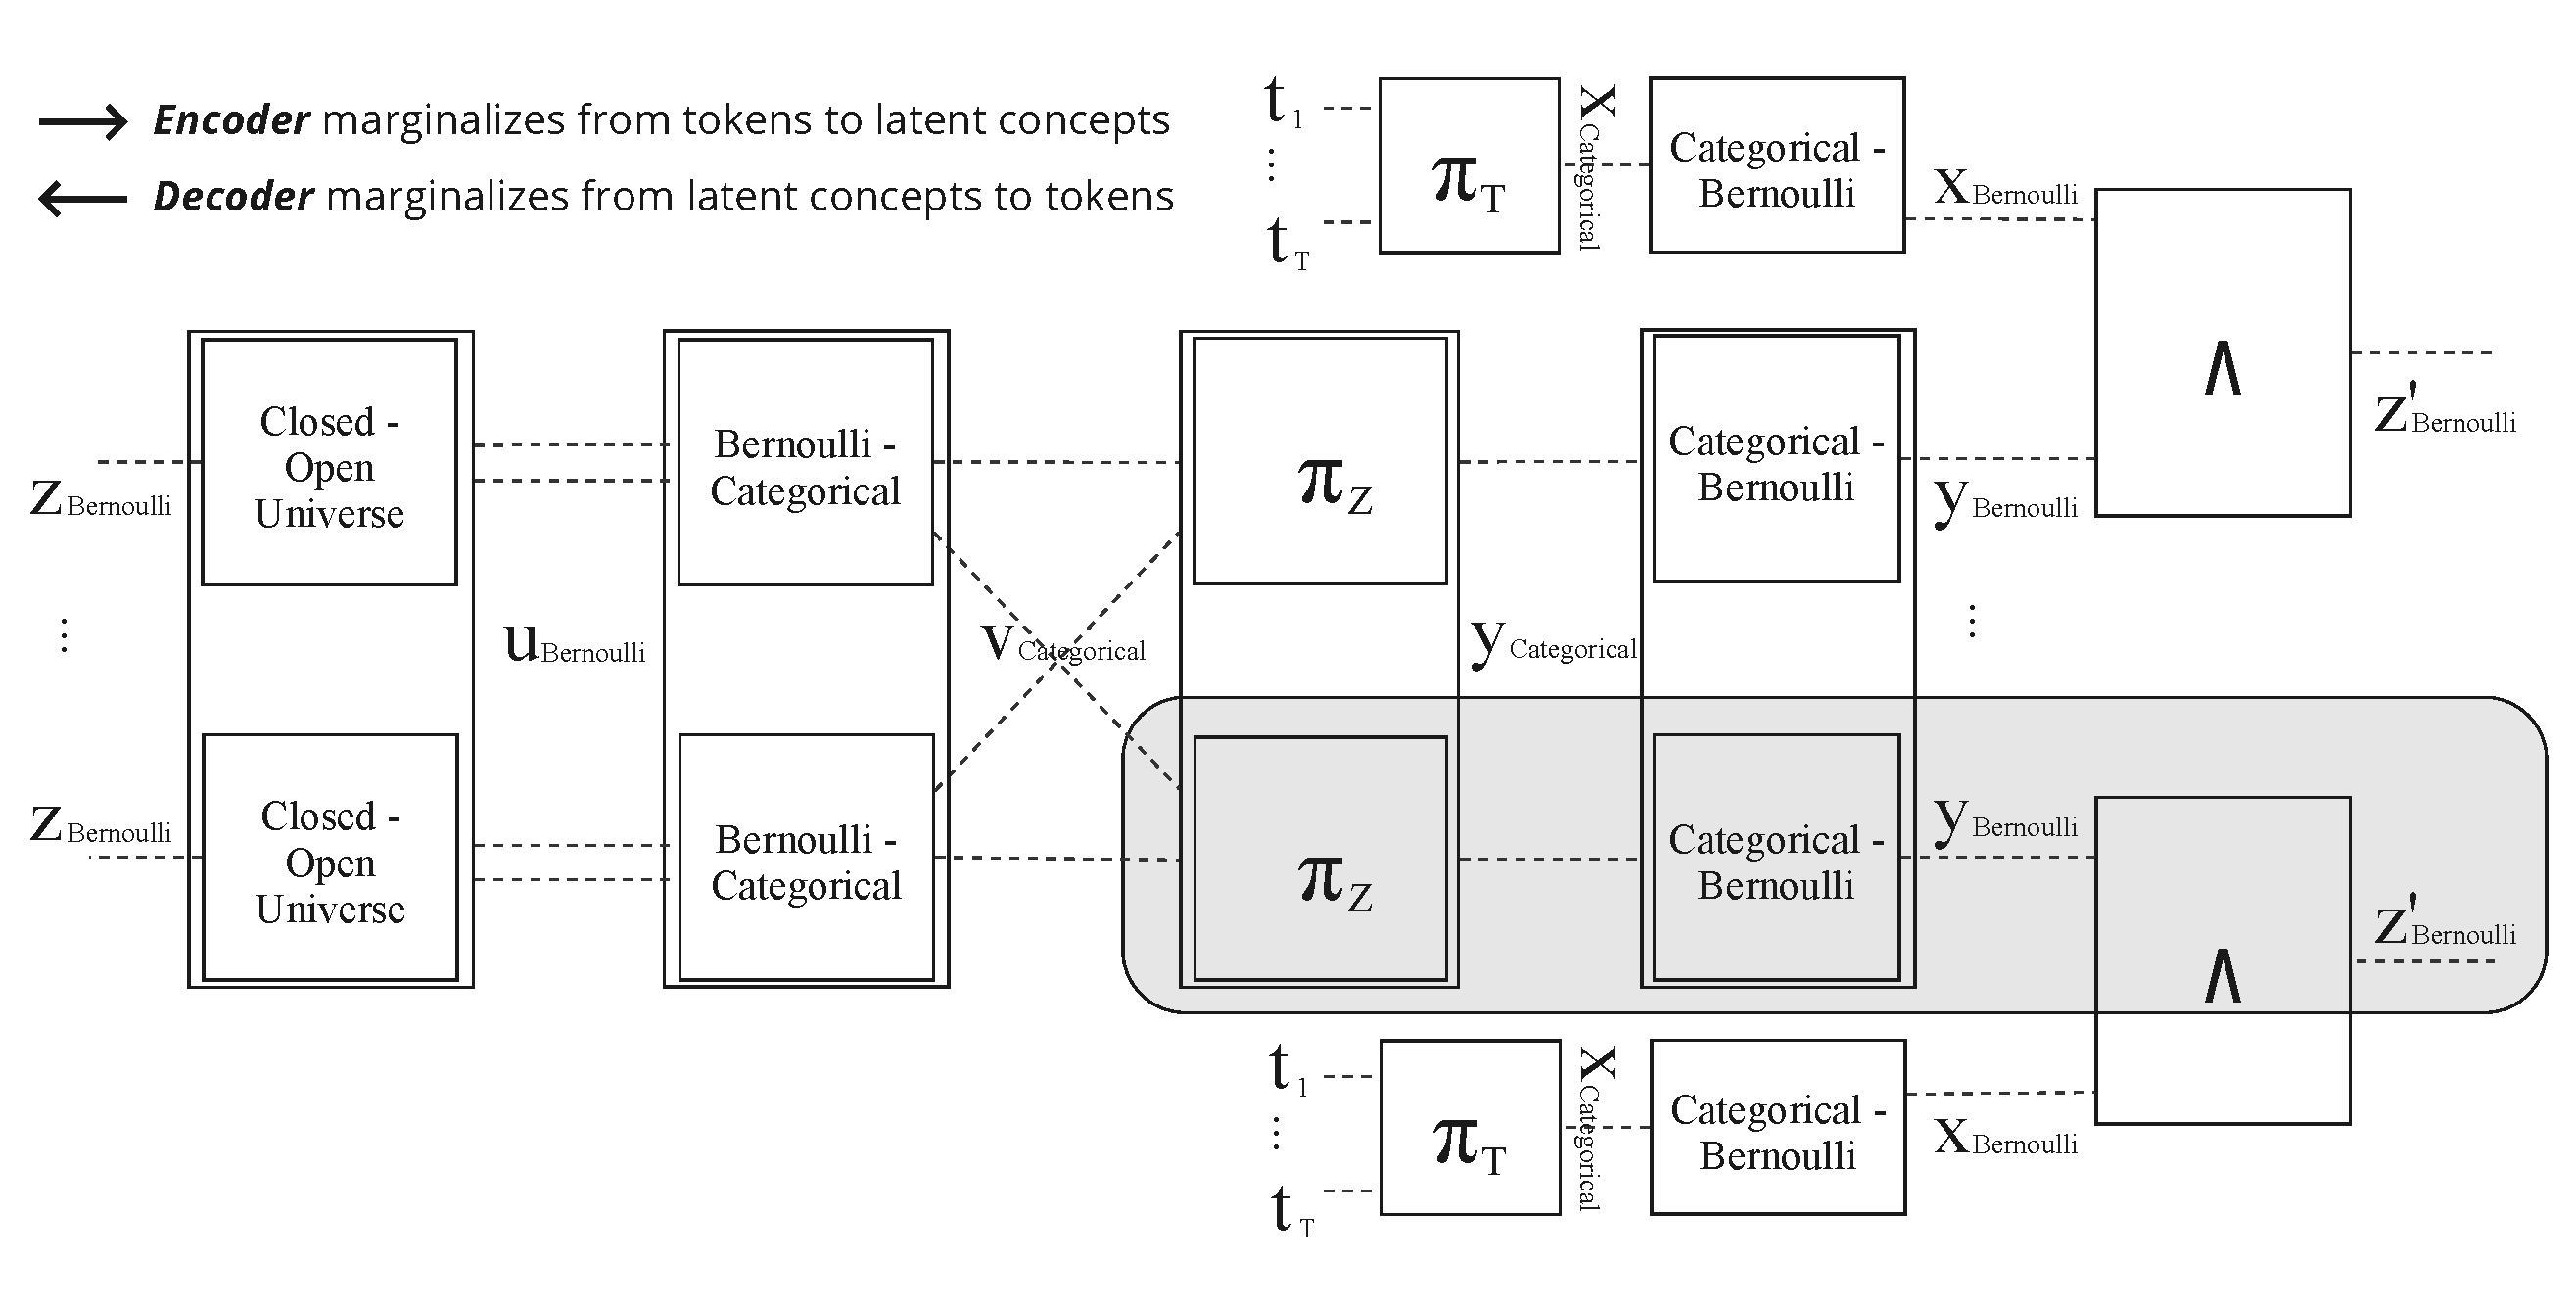
\includegraphics[width=\textwidth]{figures/transformer_factor_graph.pdf}
    \caption{A single layer of the inductive transformer production represented as a factor graph.}
    \label{fig:factor-graph-for-inductive-transformer}
\end{figure}

To begin designing our model with inductive bias, we step through a sequence of sampling operations representing a single path through one simplified decoder layer.  The $\land$ on the right side of figure \ref{fig:factor-graph-for-inductive-transformer}, is an ``AND'' activation function, detailed in appendices \ref{eq:encoder-and},\ref{appendix:decoder-and}, and \ref{appendix:log-probability-and}. When activated by $z'$, it must activate both of its child variables $x$ \emph{AND} $y$. $x$ then activates $\pi_T$ which is a categorical choice over tokens $t \in T$. When activated by the $\land$, $\pi_T$ ``rolls a die'' to choose a token.  Because it generates a ``terminal symbol'', $\pi_T$ corresponds to the residual (or ``skip'') connections in the vanilla transformer which connect internal layers to a position in the data (more on this in appendix \ref{appendix:residual-connection}). The $\land$ also activates the child variable $y$ which activates $\pi_Z$. When activated by the $\land$, $\pi_Z$ chooses a $\land$ in the layer below.  In summary, this simplified production generates one token \emph{and} chooses to activate one of the productions in the layer below.  A path through multiple layers of strongly connected productions can generate a coherent distribution over possible token sequences.  We will refer to this kind of sub-network as a ``concept''.  We will discuss the closed-open universe and categorical-Bernoulli factors later, and in full detail in appendices \ref{appendix:Open-Closed-Universe} and \ref{appendix:Categorical-To-Bernoulli}.

There are many directions for variation and expansion of this inductive bias: (1) The definitions of $\pi_T$ and $\pi_Z$ can be expanded as is shown in appendix \ref{appendix:vanilla-self-attention} when we incorporate (relative) position to implement an attention mechanism which closely resembles the XL-Transformer~\cite{dai2019transformerxl}.  (2) Because it makes a categorical choice over tokens, this production generates embedding vectors that represent one token per dimension, but this will be expanded to represent vanilla sparse semantic distributions in appendix \ref{appendix:from-indicator-to-embedding}.  (3) The production could allow for each $\pi_Z$ to (jointly) choose \emph{two} or more productions and/or each $\pi_T$ to choose two or more tokens. (4) An inductive bias for context-free grammar could be designed in order to prefer syntactically correct computer code.  Perhaps a production could also be designed to favor the generation of formally correct statements and/or steps in an axiomatic system such as Zermelo–Fraenkel set theory~\citep{hrbacek2017introduction}. (5) Other biases could be introduced by making use, for instance, of the ontological architectures explored in~\cite{gruber1993translation, gruber1995toward}. For space and clarity, we initially content ourselves with presenting our methodology for designing inductive bias for the simplified example in figure \ref{fig:factor-graph-for-inductive-transformer}.

Although our simple production resembles probabilistic generative grammars which have generally been used to model the generation of a sentence, given the penchant in biological evolution for preservation and reuse of existing structures, we see no reason to presume that this production as a modeling building block would stop being used at the end of a sentence.  This form of production also seems to naturally fit what humans call outline form for books, composition forms in music such as the sonata~\citep{Lerdahl1983}, and the hierarchical categories and attributes expressed in symbolic systems such as the Dewey decimal system and relational databases where a particular $\pi_T$ can be viewed as modeling a relation between a subject $\pi_T$ above and an obbject $\pi_T$ below.

In table~\ref{tab:rosetta}, we compare the vanilla transformer~\citep{vaswani2017attention} to the inductive transformer layer by layer.

\setlength{\extrarowheight}{5pt}
\begin{table}[H]
    \centering
    \begin{tabular}{p{0.13\textwidth}>{\raggedright\arraybackslash}p{0.29\textwidth}p{0.49\textwidth}}
      \textbf{Layer Type} & \textbf{Vanilla Transformer}   &   \textbf{Inductive Transformer}   \\
      \hline
      Self-attention & $y_i = \sum_j \omega_{i,j} v_j$, where \qquad $\omega_{i,j} = \textrm{Softmax}(q_i k_j^T)$ & We do not modify the attention layer, we only reinterpret it as marginalizing a statistical production. See appendix~\ref{appendix:vanilla-self-attention} \\
      \hline
      Add \& norm & Sum the residual connections and the outputs from the attention layer below.  &  Marginalization of the ``$\land$'' sums the the token activations output from $\pi_T$ with the attention activations from $\pi_Z$. See appendix~\ref{appendix:log-probability-and}\\
      \hline
      Residual connections & Connections between the input data and internal layers & Generative grammar-style model where every non-terminal must generate at least one terminal. See appendix \ref{appendix:residual-connection} \\
      \hline
      Encoder-decoder connections & Output of the encoder inputs to every decoder layer & When we detail forward and backward marginalization in the model, we will see each layer of the encoder should provide marginals to the corresponding decoder layer. See appendix \ref{appendix:connecting-encoder-to-decoder}\\
      \hline
      Feed-forward & Multiple fully-connected nonlinear layers e.g. ReLu's & Marginalizes the posterior log probability of the categorical-Bernoulli, open-closed universe, and Bernoulli-categorical factors. See section~\ref{section:open-closed-universe} \\
      \hline
    \end{tabular}
    \caption{Comparison of Vanilla and Inductive Transformer Layers}
    \label{tab:rosetta}
\end{table}

As we discuss in table \ref{tab:rosetta} above and detail in appendix \ref{appendix:vanilla-self-attention}, we strive for a close correspondence between the equations for the vanilla attention mechanism and the equations we derive by marginalizing our attention production.

Similarly, the correspondence between the $\land$ factor and the add \& norm layers in the vanilla transformer is strongly suggested by the fact that these layers are where the residual connections get combined with the activations from the layer below.  Furthermore there is a close mathematical correspondence between the implementation of the $\land$ in the log probability domain and the add \& normalization operation (see further details in appendix~\ref{appendix:vanilla-self-attention}).

Much is therefore the same.  Where do the inductive and vanilla transformers differ?  There is one difference in how the encoder of the inductive transformer should connect to the decoder. See appendix \ref{appendix:connectivity} for more details.

More substantially, let us look at the feed-forward layer.  In the vanilla transformer, the feed-forward layer applies the same operation (essentially a multi-layer perceptron) to each embedding vector coming into it.  The vector at each position is processed through its own perceptron independent of the vectors at other positions, but the same weights are employed at every position -- these independent operations are identical to one another.  Similarly, when we derive the inductive transformer, we find by process of elimination that the closed-open-universe factor and the Bernoulli-to-categorical factor (with its subsequent layer norm) must be somehow performed by the feed-forward layer in the vanilla transformer in order for there to be a tight correspondence between the two approaches.  Miraculously, when we implement inference as marginalization on a model comprised of layers of productions, the same independence of columns as well as the subsequent layer add \& norm falls out of the inductive transformer derivation.  In essence we recover the exact same conditional independencies in the factor graph for the inductive transformer as are present in the vanilla transformer, and they fall out not as the result of tinkering, but as the result of theory where our guiding force was to apply the constraints imposed by the production while also preventing the $O()$ for any of our factors from being exponential!

This is highly suggestive of a strong correspondence.  There is an important difference between the approaches, however.  In the inductive transformer we are precisely defining the functions for our ``feed-forward'' layer to implement~\ref{appendix:activation-functions}.  In the vanilla transformer these same functions must be learned from data.  This suggests that perhaps we ought to pretrain the feed-forward layers of vanilla transformers with synthetic data designed to teach them how to be an open-closed-universe-Bernoulli-to-categorical factor. Conversely, as we relax this layer of the inductive transformer back to being a vanilla feed-forward layer, we recover the vanilla transformer.


\section{Inference in the Inductive Transformer}

In this section, we will start to see that we can understand inference in a transformer not just as predicting the next token given previous tokens, but as inferring ``forward'' into a latent space of concepts and then ``backwards'' to predict tokens in the token window.

Determining the certainty of latent concepts in the model given the input data is, in general, an underdetermined inverse problem.  When the probability distribution of a model can be represented by a directed acyclic graph, then forward-backward marginalization of the model is exact and computationally efficient~\cite{10.5555/779343.779352}.

Although our highly connected multilayer neural network may appear to be a cyclic graph, in fact the model represented by concatenation of our productions is a tree.  It is only the transformation from an open-universe model to a closed-universe model, discussed in detail in appendix ~\ref{appendix:Open-Closed-Universe} that makes the model appear to have loops.

The conditional distribution for the inductive transformer decoder in figure \ref{fig:factor-graph-for-inductive-transformer} is,
\begin{align}
\label{eq:rho_marginalized_out}
p(z|u)p(u|v_{\text{Categorical}})p(v_{\text{Categorical}}|y_{\text{Categorical}})p(y_{\text{Categorical}}|y)p(t|x_{\text{Categorical}}) \nonumber \\
p(x_{\text{Categorical}}|x)p(x, y|z')p(z').
\end{align}

where $\pi_T = p(t|x_{\text{categorical}})p(x_{\text{categorical}}|x_{\text{Bernoulli}})$ and $\pi_Z = p(v_{\text{categorical}}| y_{\text{categorical}})p(y_{\text{categorical}}|y)$.  We represent Bernoulli variables with the subscript ``Ber''  or with no subscript.  We use the subscript ``categorical'' to denote categorical distributions which collect multiple Bernoulli variables into a single joint variable across a layer of activations. This turns out to be important in order to avoid exponential computational complexity in certain layers.  See appendices~\ref{appendix:Bernoulli-Categorical} and~\ref{appendix:Categorical-To-Bernoulli} for more details.  

As we input a prompt, rightward marginalization in figure~\ref{fig:factor-graph-for-inductive-transformer} computes activations at each layer of the \emph{encoder}. Conditioned on the concepts activated in the encoder, leftward marginalization through the factor graph infers the \emph{decoder} activations.  During leftward marginalization, tokens are sampled from the probabilities (activations) in the $\pi_T$'s.  

Now we derive the equations for marginalizing the inductive transformer.  A transformer architecture may contain an encoder and/or a decoder.  We start with the decoder. Inference in a layer of the decoder marginalizes the conditional distribution in equation~\ref{eq:rho_marginalized_out}.  To massively reduce the computational complexity of the marginalization, we push each summation as far to the right as we can,

\begin{align}
p(z) &= \sum_u p(z|u)\sum_{v_\text{categorical}}p(u|v_{\text{Categorical}})\sum_{y_\text{categorical}}p(v_{\text{Categorical}}|y_{\text{Categorical}}) \nonumber \\ 
&\quad\quad \cdot \sum_y p(y_{\text{Categorical}}|y) \sum_{x_\text{categorical}} p(t|x_{\text{Categorical}})\sum_x p(x_{\text{Categorical}}|x) \sum_{z'}p(x, y|z')p(z').
\end{align}

Some of the conditional distributions in this equation are,

\begingroup
\addtolength{\jot}{1em}
\begin{align}
    p(x, y|z') &= \delta(z'_{\text{Ber}}-\land(x_{\text{Ber}}, y_{\text{Ber}})), \\
    p(v_{\text{Categorical}}|y_{\text{Categorical}}) &= W_{v,y}, \\
    p(t_{\text{Categorical}}|x_{\text{Categorical}}) &= W_{t,x}.
\end{align} 
\endgroup

where $W$'s are learned weight matrices. The \emph{encoder} marginalizes in the opposite direction of the decoder, with conditional distributions that impose the same joint constraints on adjacent variables.  \emph{Detailed and pedagogical equations for each summation are provided in appendix}~\ref{appendix:activation-functions}.


\section{Illustrative Example}

Before concluding, let's zoom into a tiny component of a larger inductive transformer to see the real-world operation in detail.

\subsection{Model weights and activations}

\begin{figure}[H]
    \begin{center}
    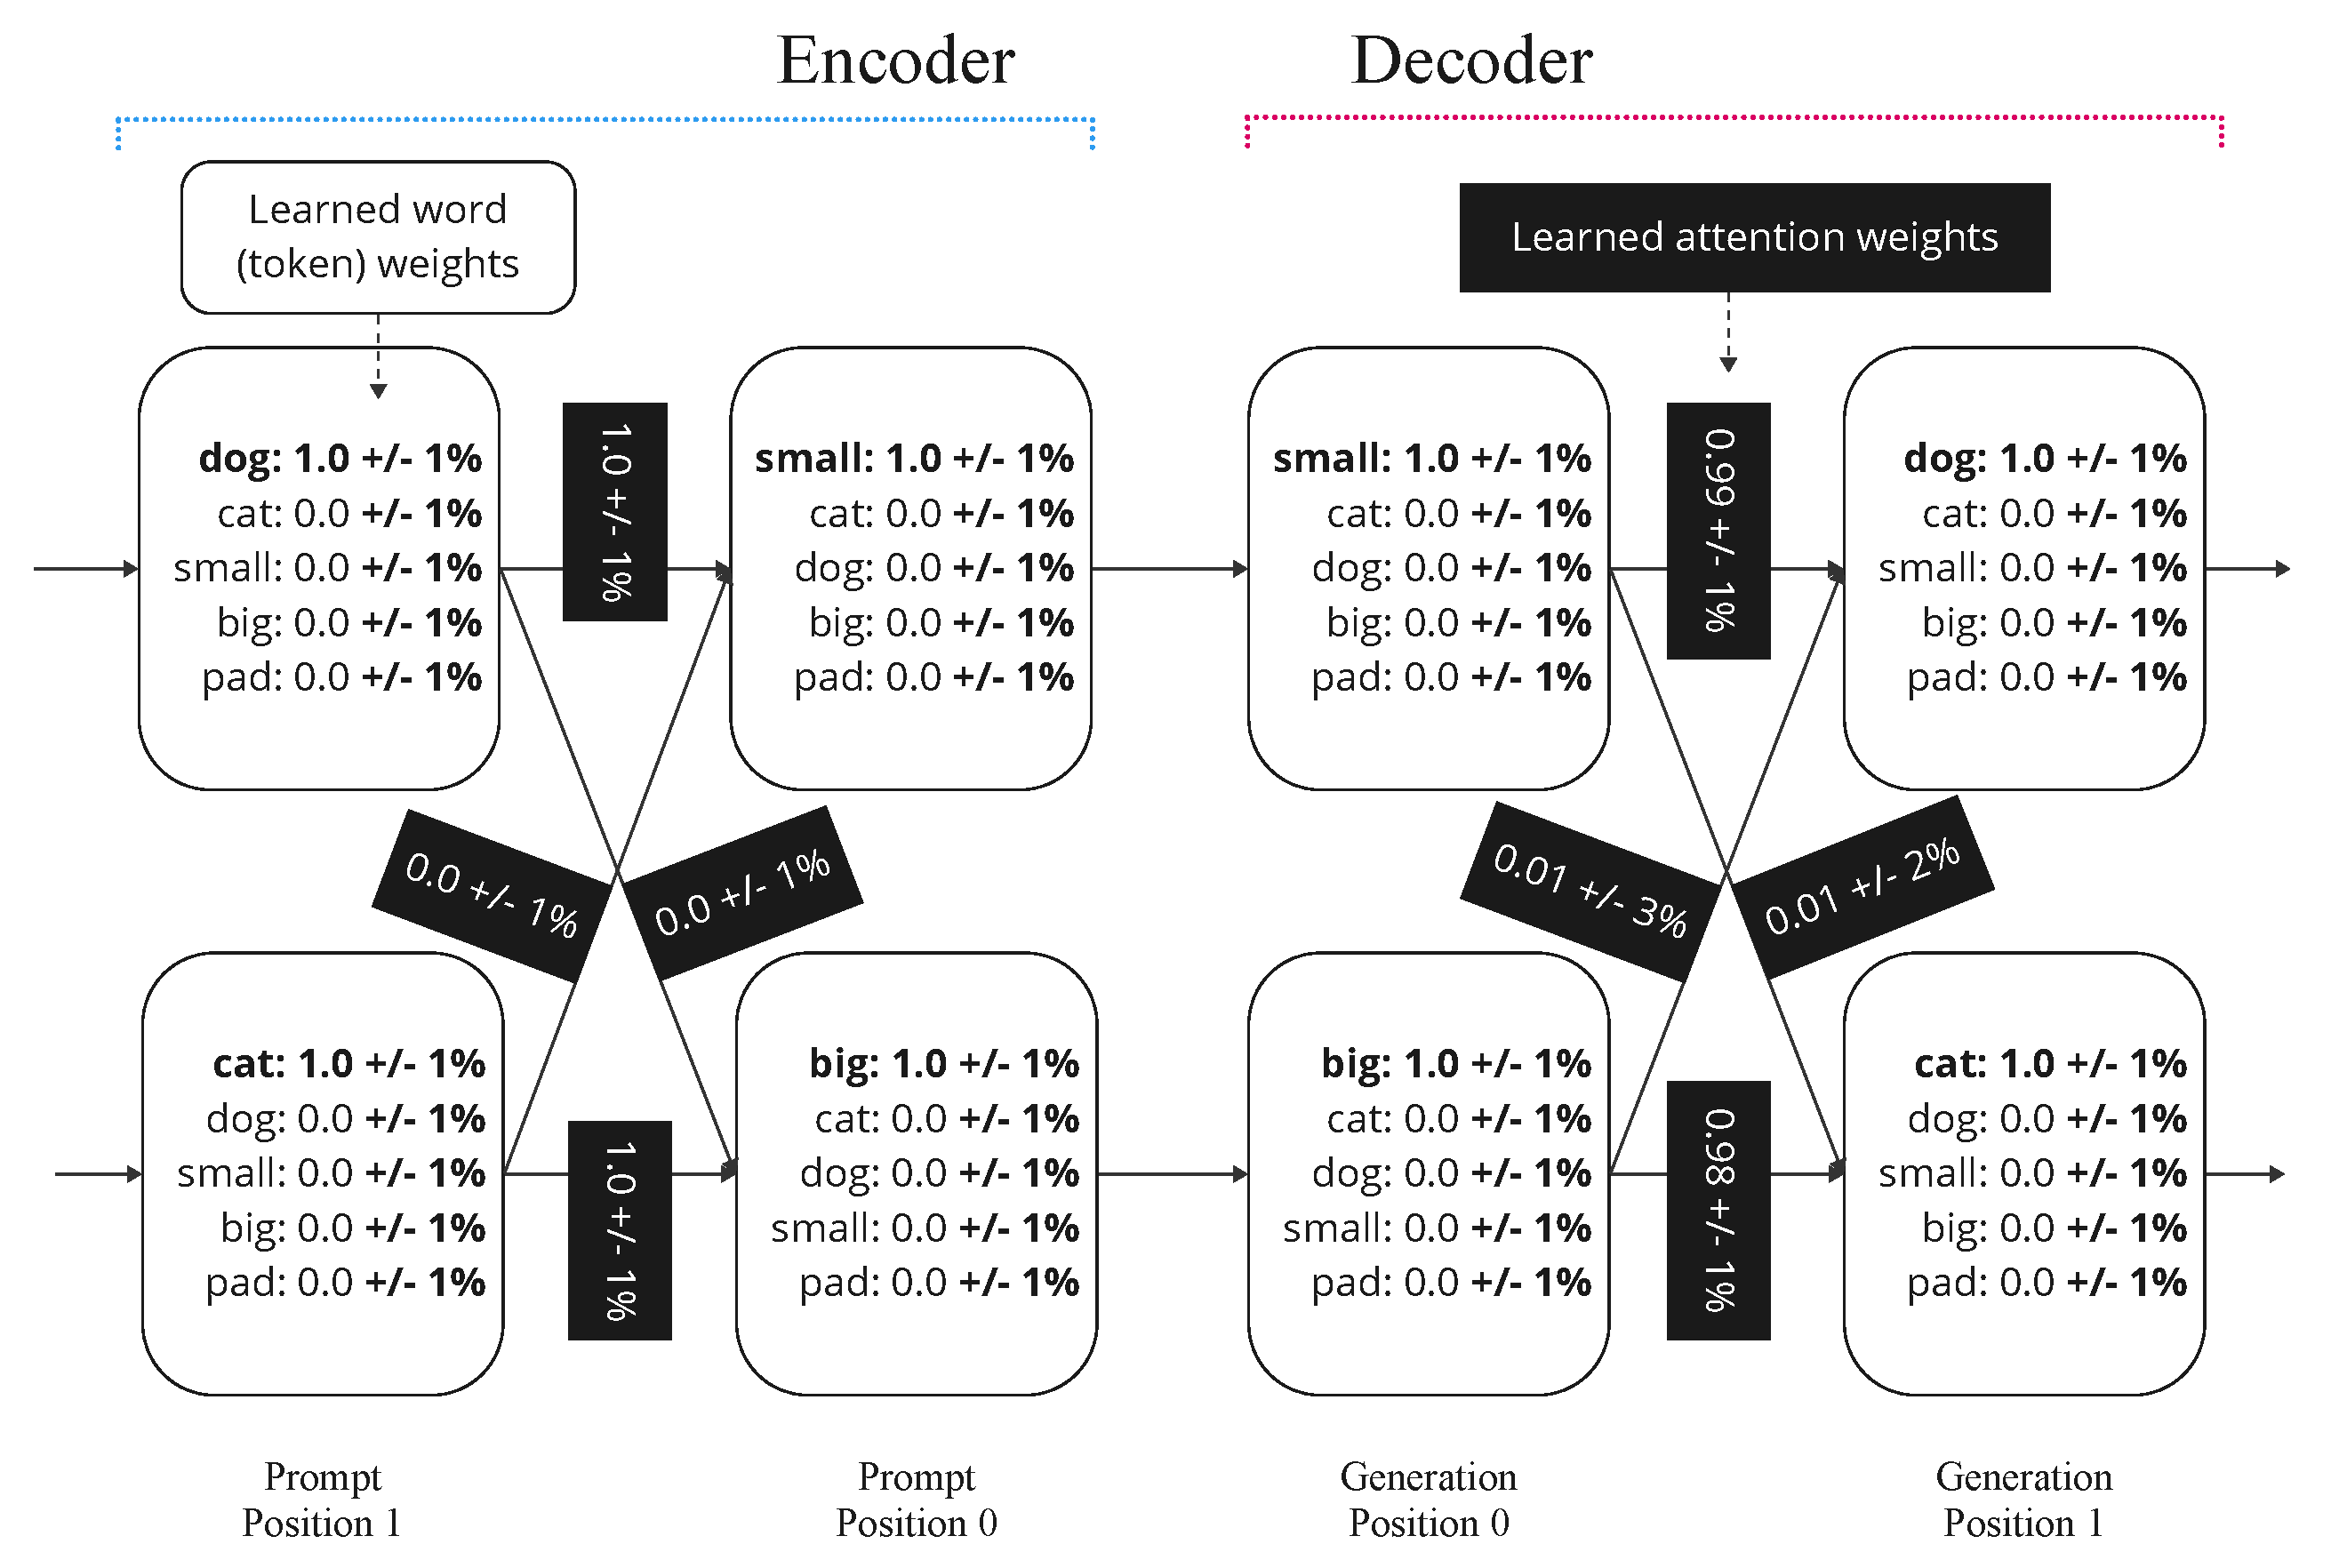
\includegraphics[width=\textwidth]{figures/results_factor_graph_with_weights.pdf}
    \caption{Learned Weights in the Inductive Transformer. The learning is highly reproducible. In a hundred different learning runs, the variance of each learned weight is generally less than 1\%. The attention $\pi_Z$ weights are in white with black background while the token $\pi_T$ weights are black on white, next to their corresponding vocabulary words.}
    \label{fig:result-weights}
    \end{center}
\end{figure}

In order to illustrate the weights of the model on a single page, we trained a small two-layer section of the model with two-token positions in the training text window.  We use a maximally sparse embedding representation described in more detail in appendix \ref{appendix:from-indicator-to-embedding}.  This highly simplified instance of our inductive transformer generates a single token per production and therefore a single token per layer. In other words, $P$ tokens in the data window needs to be explained away by $P$ layers in this version of the inductive transformer.  If we desire a model architecture that can compress more tokens into fewer layers, we adjust the production so that a single layer is able to generate more than a single token.

The model was implemented in PyTorch and trained with back-propagation using the Adam optimizer~\citep{NEURIPS2019_9015, kingma2017adam}.  In figure~\ref{fig:result-weights} we see each learned weight with its variance across a hundred training runs.

\subsection{Prompting and Generation}

How does prompting and generation happen in the inductive transformer?  Having been trained on data phrases like ``big cat'' and ``small dog'', when we prompt the model with the word ``big'', and having converged to the weight values shown above, the system generates the phrase ``big cat''.  When we prompt the model with the word ``small'' it generates the phrase ``small dog''.  Given its hierarchical categorical nature, there is a sense in which the encoder conceptualizes ``small'' and ``big'' as kinds or modifiers of ``dogs'' and ``cats''.

\begin{tabular}{ccc}
\hline\hline
Prompt & Generation &  \thead{Percentage \\ of Generations} \\[1ex]
\hline\hline
``big'' & ``big cat'' & 100\% \\
``big'' & ``big dog'' & 0\% \\
\hline
\end{tabular}
\quad\quad\quad
\begin{tabular}{ccc}
\hline\hline
Prompt & Generation &  \thead{Percentage \\ of Generations} \\[1ex]
\hline
``small'' & ``small dog'' & 100\% \\
``small'' & ``small cat'' & 0\% \\
\hline
\end{tabular}

\subsection{Identifiability}

The inductive transformer strongly organizes the concepts it learns; It organizes its concepts (1) the same way as the model that generated its training data, and (2) the same way every time.  This novel training repeatability is a consequence of the strong inductive bias.

In our context, ``identifiability'' means the ability for a learning model to receive instructional data from a teacher model, and repeatably learn to mirror the teacher model's structure.  To determine if our model is identifiable in this sense, we follow these steps:

\begin{enumerate}
    \itemsep -0.25em 
    \item Create a \emph{forward model} with weights set to particular values.
    \item Generate tokens (\emph{generated data}) from this forward model.
    \item Copy the forward model to create an \emph{inverse model} with randomly initialized weights.
    \item Use the generated data from the forward model to train the inverse model.
    \item Compare the (learned) weights in the inverse model to the weights in the forward model.  If the weights in the inverse model converge to the same values as the corresponding weights in the forward model, then we say that the model is identifiable.
\end{enumerate}

We see in figure \ref{fig:result-weights} that when repeatedly trained on the same data, the inductive transformer repeatably learns to position the same concepts in the same places within the model. This is repeatable with only a small nudge in one corner of the model to break symmetry. On larger data sets, longer range correlations in the data ensure this symmetry breaking.

The identifiability in the inductive transformer is reminiscent of the fact that for a wide range of concepts, different humans from diverse backgrounds learn to localize particular concepts at the same positions in their brains~\citep{DBLP:journals/nature/HuthHGTG16, li2023large, geva-etal-2021-transformer, merlin2022language}.

% \subsection{Rejection of Low Quality Data}

% \begin{table}[H]
%     \begin{center}
%     \begin{tabular}{ccc}
%         \hline\hline
%         Training Data &  \thead{Percentage} \\[1ex]
%         \hline\hline
%         ``dog dog'' & 10\% \\
%         ``small dog'' & 40\% \\
%         ``big cat'' & 50\% \\
%         \hline
%     \end{tabular}
%     \quad\quad\quad
%     \begin{tabular}{ccc}
%         \hline\hline
%         Free Generations After Training &  \thead{Percentage} \\[1ex]
%         \hline\hline
%         ``small dog'' & 44.4\% \\
%         ``big cat'' & 55.6\% \\
%         \hline
%     \end{tabular}
%     \caption{After training, the model only reflects the high quality training data, e.g. ``small dog'', and rejects the low quality training data, e.g. ``dog dog''.}
%     \end{center}
%     \end{table}

\subsection{Controllability}

Now we demonstrate that we can delete concepts in the inductive transformer, so that the model will no longer generate text from those concepts. Suppose the section of the model shown in figure~\ref{fig:result-weights} was trained with the three sentences ``big cat'', ``big dog'', and ``small dog'', so that while everything else stays the same, the $\pi_Z$ in the `big' production learns weights $[0.5, 0.5]$ and when prompted with the word ``big'', the model generates outputs:

\begin{table}[H]
\begin{center}
\begin{tabular}{ccc}
\hline\hline
Prompt & Generation &  \thead{Percentage \\ of Generations} \\[1ex]
\hline\hline
``small'' & ``small dog'' & 100\% \\
``small'' & ``small cat'' & 0\% \\
\hline
\end{tabular}
\quad\quad\quad
\begin{tabular}{ccc}
\hline\hline
Prompt & Generation &  \thead{Percentage \\ of Generations} \\[1ex]
\hline
``big'' & ``big cat'' & 50\% \\
``big'' & ``big dog'' & 50\% \\
\hline
\end{tabular}
\caption{After training, the model accurately reflects the training data.}
\end{center}
\end{table}

If we lesion the connection between the ``big'' production and the ``dog'' production, then the model can only say ``big cat'' and ``small dog'', and will no longer say ``big dog'':

\begin{table}[H]
\begin{center}
\begin{tabular}{ccc}
\hline\hline
Prompt & Generation &  \thead{Percentage \\ of Generations} \\[1ex]
\hline\hline
``small'' & ``small dog'' & 100\% \\
``small'' & ``small cat'' & 0\% \\
\hline
\end{tabular}
\quad\quad\quad
\begin{tabular}{ccc}
\hline\hline
Prompt & Generation &  \thead{Percentage \\ of Generations} \\[1ex]
\hline
``big'' & ``big cat'' & 100\% \\
``big'' & ``big dog'' & 0\% \\
\hline
\end{tabular}
\caption{Prompted generations from the model where we broke the connection between ``big'' and ``dog''.}
\end{center}
\end{table}

This demonstrates that the inductive transformer can learn causal relationships between connected sub-networks of productions. Such a sub-network can generate text to represent its concept with many different but synonymous token sequences. Given the very close mathematical similarity between inductive and vanilla transformers, it seems very likely that vanilla transformers also form concepts.  Although concepts may not be highly localized or organized in the vanilla transformer, they could increasingly be so if we add further inductive bias. Furthermore this suggests that the ``emergent" capabilities of large language models as they scale~\citep{wei2022emergent} may be the result of adding additional ``layers'' of concepts that provide higher levels of abstraction.

Model controllability also has practical applications.  It could, for example, make it safer and simpler to share learned weights between models. With concept controllability, after training models on new data and/or reinforcements, people or organizations who exchange weight updates could verify and control the concepts they are sharing across models. Controllability could also make it possible to control concepts in a model rather than spending far greater effort to scrub training data, and could be used to help scrub data by identifying particular concepts with particular sections of text. Finally, concept controllability could also be utilized to help enhance AI alignment.



\section{Discussion}

Our theory of inductive transformers makes two predictions.  The first is that training foundation models with data sets that instantiate a particular inductive bias can help unlock a range of new abilities.  To do this one could generate synthetic data from, for example, the model we described here, and use this synthetic data within the overall mix of training data for a foundation model~\citep{akyurek2020learning}. The general principle is that we could train useful inductive biases into a transformer before or in concert with training on natural language data.  

The second prediction is that training data for inductive bias can be replaced or augmented by directly designing the inductive bias into the activation functions and connectivity of the model.  We showed in table \ref{tab:rosetta} that most layers of the inductive transformer are identical to the vanilla transformer, and we only need specialize the feed-forward layer to gain additional inductive bias.

Foundation models pretrained with inductive bias data and/or designed with inductive bias based on recursive productions could be smaller, more modular, and able to develop more advanced abilities.  

% For inclusion once review anonymity is lifted:
% \subsubsubsection{\textbf{Acknowledgements.}}
% The authors are grateful for funding in part by DARPA Contract FA8750-14-C-0001.  The authors are also grateful for discussions with Matt Barr, Steve Willis, and Jeff Bernstein.

% \subsubsubsection{\textbf{Authors’ contributions.}} B.V.:  conceptualization, supervision, methodology, mathematical development, writing original draft, citations, writing review and editing, pair-coding, running simulations. T.R.: mathematical development, writing review & editing, citations, pair-coding, running simulations.

%%%%%%%%%%%%%%%%%%%%%%%%

\newpage
\bibliographystyle{iclr2024_conference}
\bibliography{references}

\newpage
\appendix



\section{Connectivity in the Inductive Transformer}\label{appendix:connectivity}

\subsection{Residual Connections in Vanilla Transformer $\rightarrow$ Reduced Productions in the Inductive Transformer}\label{appendix:residual-connection}

Transformer architectures (and other deep learning architectures) utilize residual (ie. skip) connections.  Residual connections have been empirically demonstrated to smooth the fitness landscape helping back-propagation converge:

\begin{quote}
``We find that network architecture has a dramatic effect on the loss landscape. Shallow networks have smooth landscapes populated by wide, convex regions. However, as networks become deeper, landscapes spontaneously become `chaotic' and highly non-convex, leading to poor training behavior... Skip connections cause a dramatic `convexification' of the loss landscape''~\citep{DBLP:journals/corr/abs-1712-09913}.
\end{quote}

When learning the productions for an arbitrary generative grammar, we need to prevent the learning algorithm from inserting an arbitrary number of non-terminal nodes in the chain of generations. ``Requiring
some text to be generated at each [production] step is enough for inference to remain tractable.''~\citep{malik2021generative}

These observations may be closely related.  Adding direct connections from the data to every latent activation function in the network removes an enormous number of degenerate states from the solution space.

The fact that the add \& normalize is the layer in the vanilla transformer that has residual connections to the data tells us that this is the layer that corresponds to the $\land$ in our generative production.  In appendix~\ref{appendix:log-probability-and} we expand on this correspondence.


\subsection{Connecting the Encoder to the Decoder}
\label{appendix:connecting-encoder-to-decoder}

When performing marginalization of a probability distribution represented by a directed acyclic graph, it has long been known that marginalization (probabilistic message passing) converges after a single forward pass and backward pass through the graph~\citep{pearl1988probabilistic, mackay2003information}.

The forward pass in our generative model corresponds to the encoder, and the backward pass to the decoder. Carefully tracing the forward and backward marginalizations (as we do in appendix \ref{appendix:activation-functions} on activation functions below), shows us that the inductive transformer would benefit from a slightly different connectivity between the encoder and decoder compared to a vanilla transformer.  Empirically, however, the inductive transformer may perform satisfactorily without all of these connections.

\begin{figure}[H]
\centering
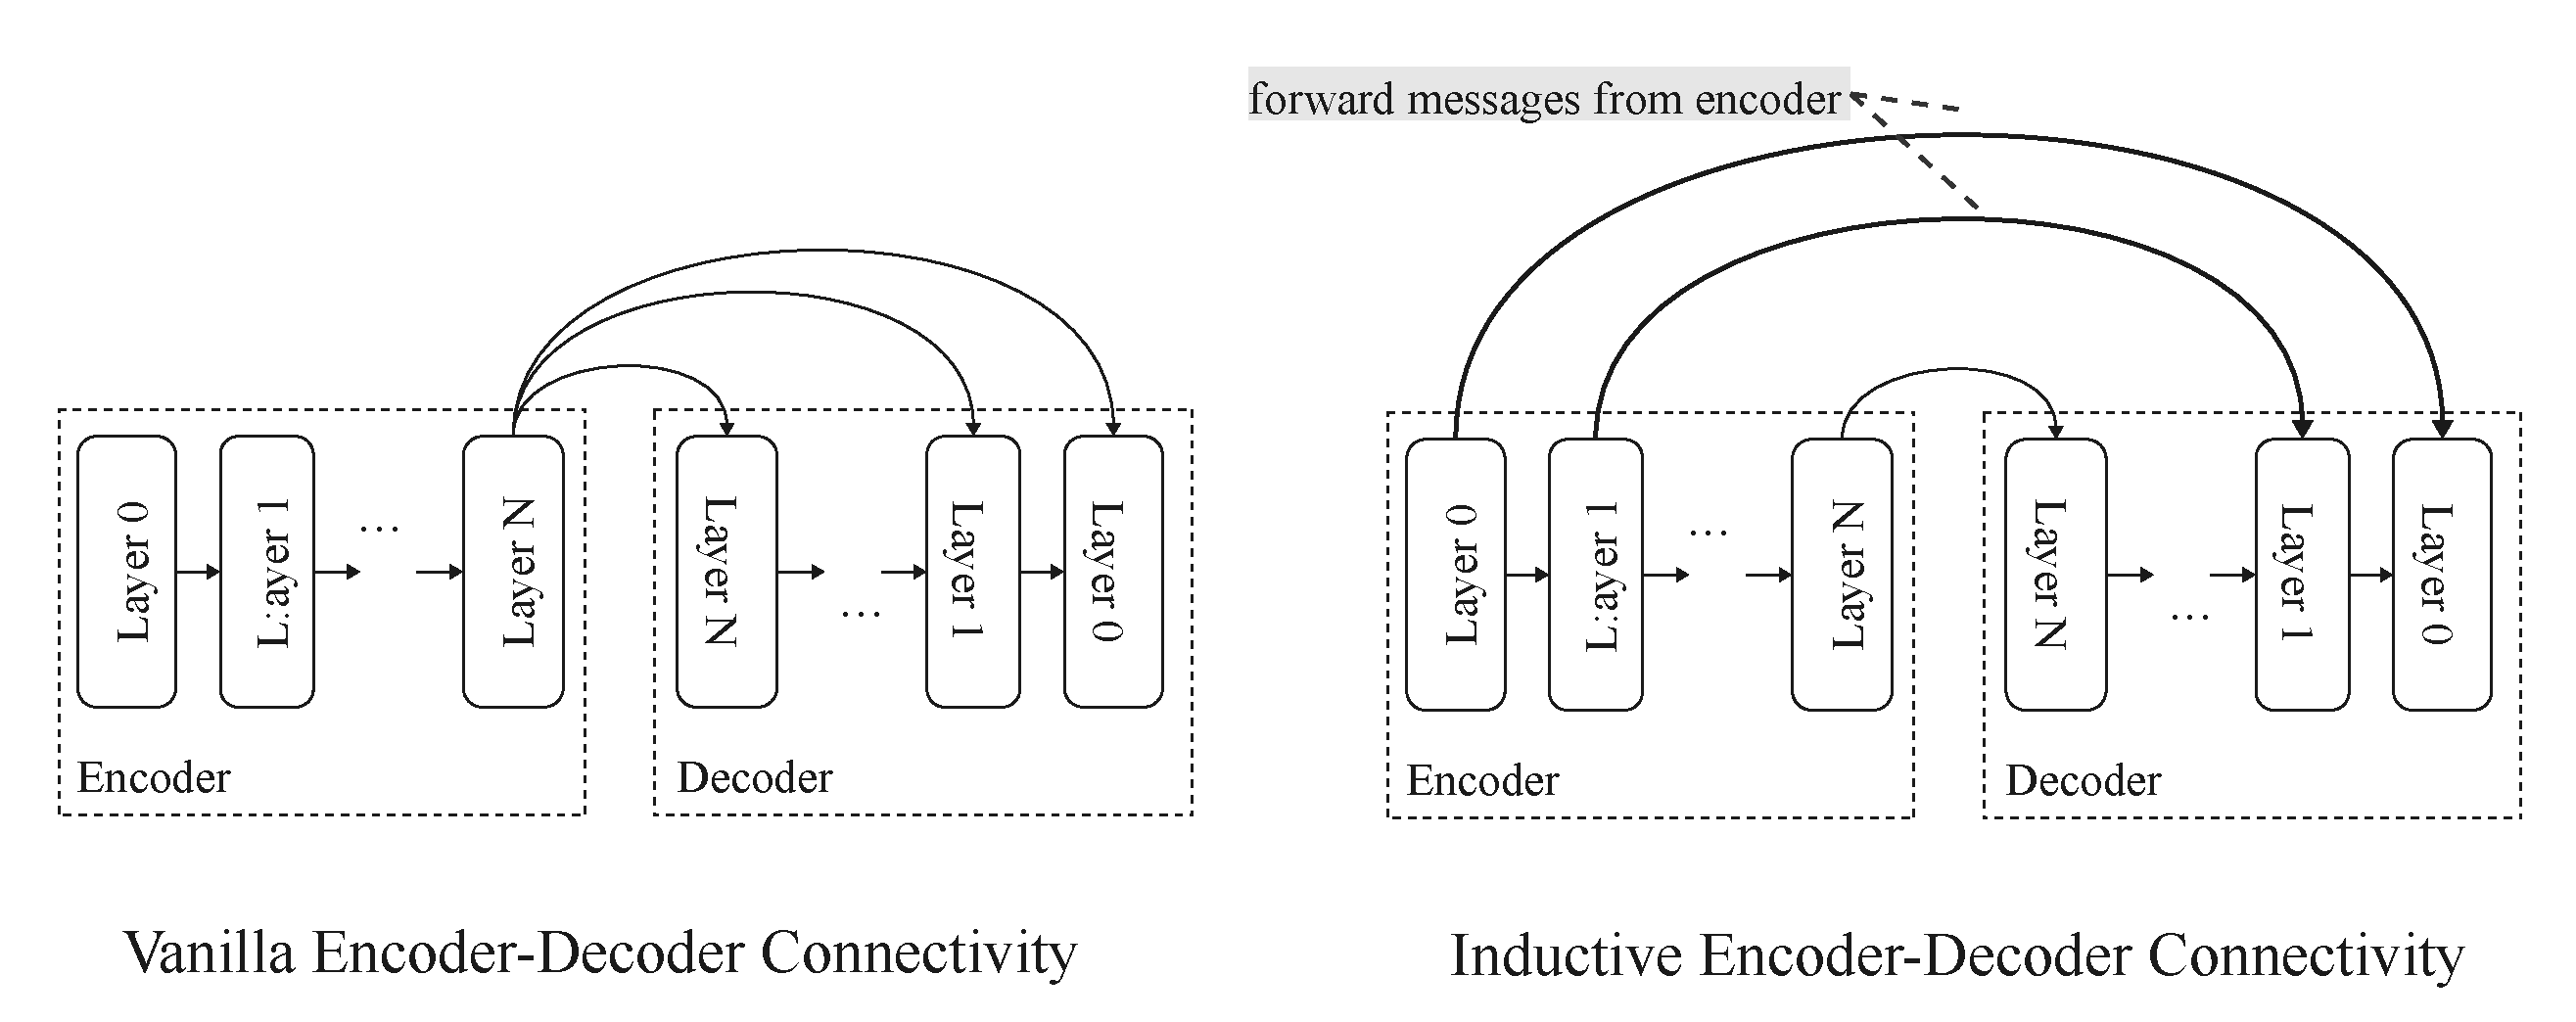
\includegraphics[width=\textwidth]{figures/inductive-encoder-decoder-connectivity.pdf}
\caption{How the Connectivity from Encoder to Decoder Differs in the Inductive Transformer.}
\label{fig:logical-encoder-decoder}
\end{figure}


\section{Activation Functions}\label{appendix:activation-functions}

\begin{figure}[H]
    \centering
    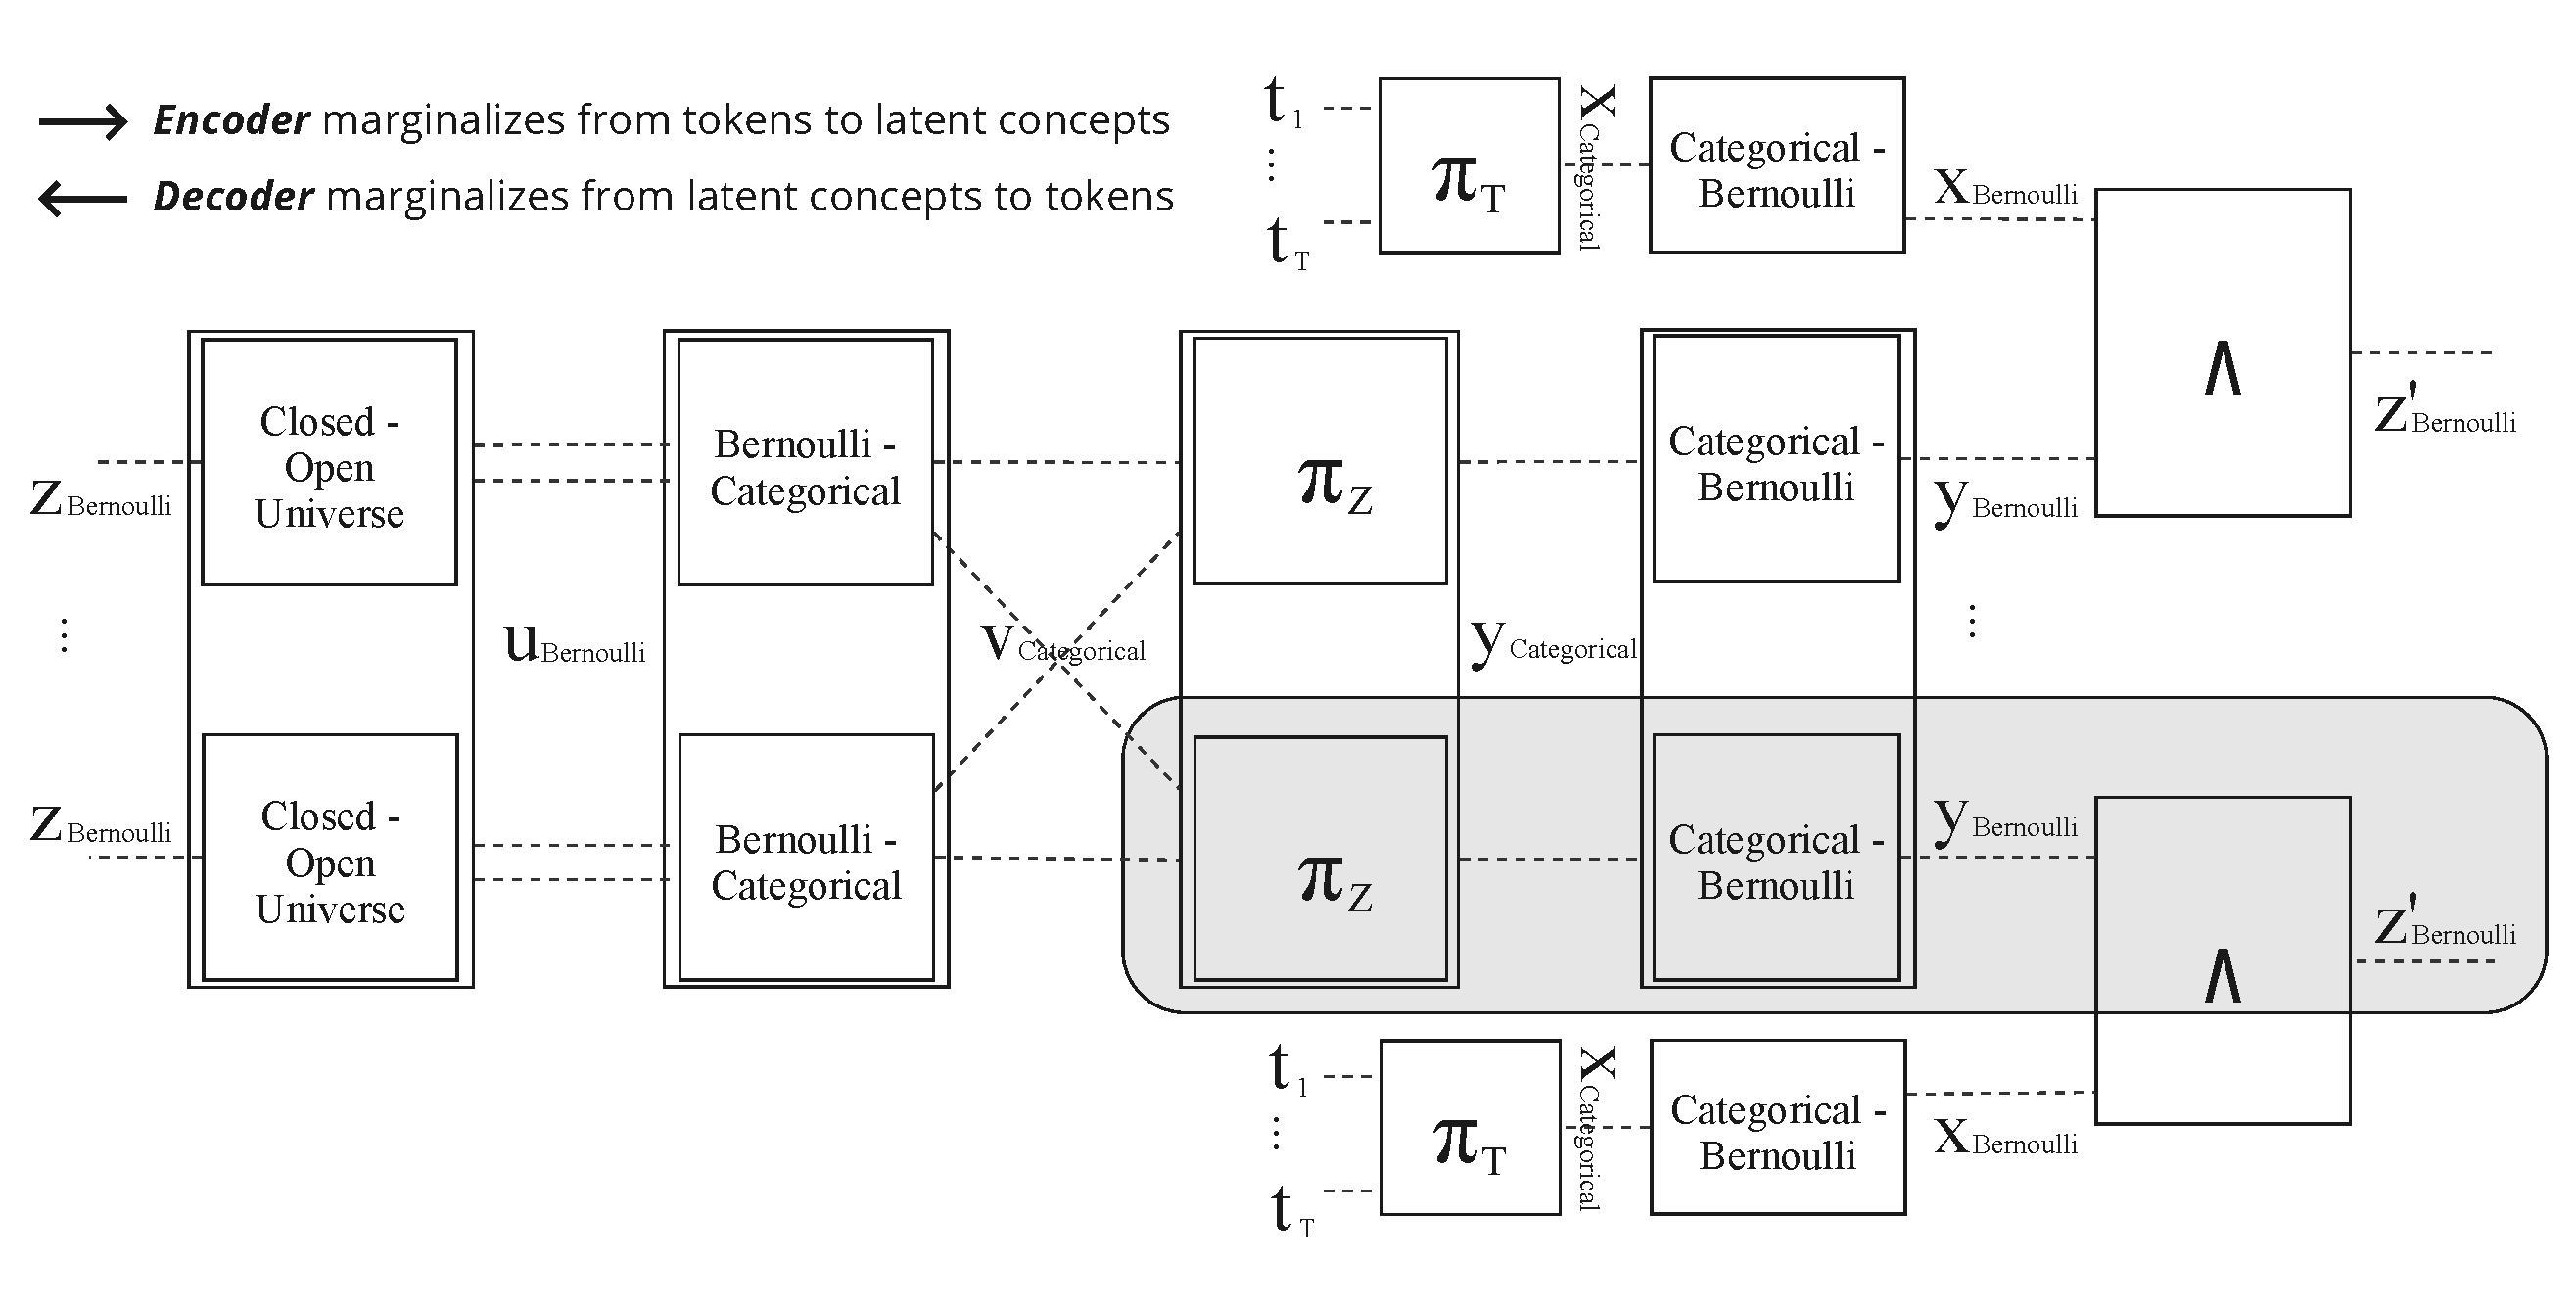
\includegraphics[width=\textwidth]{figures/transformer_factor_graph.pdf}
    \caption{Factor Graph For Inductive Transformer}
    \label{fig-appendix:factor-graph-for-inductive-transformer}
\end{figure}

The sequence of marginalization operations previously mentioned in section~\ref{section:inductive-transformer-model} correspond to layers in the inductive transformer. See figure~\ref{fig-appendix:factor-graph-for-inductive-transformer} for a detailed review of a single layer.
 The \emph{encoder} layers from the input towards the decoder are,
 
\begin{enumerate}
    \setlength\itemsep{0em}
    \item Closed-Open Universe
    \item Bernoulli-Categorical
    \item Attention $\pi$ and Token $\pi$
    \item Categorical-Bernoulli
    \item $\land$
    \item Repeat.
\end{enumerate}

The \emph{decoder} layers from the encoder towards the output are,
\begin{enumerate}
    \setlength\itemsep{0em}
    \item $\land$
    \item Bernoulli-Categorical
    \item Attention $\pi$ and Token $\pi$
    \item Categorical-Bernoulli
    \item Open-Closed Universe
    \item Repeat.
\end{enumerate}

We detail each layer below.

\subsection{1. The Open-Closed Universe Factor}\label{section:open-closed-universe}
 
\begin{figure}[H]
    \centering
    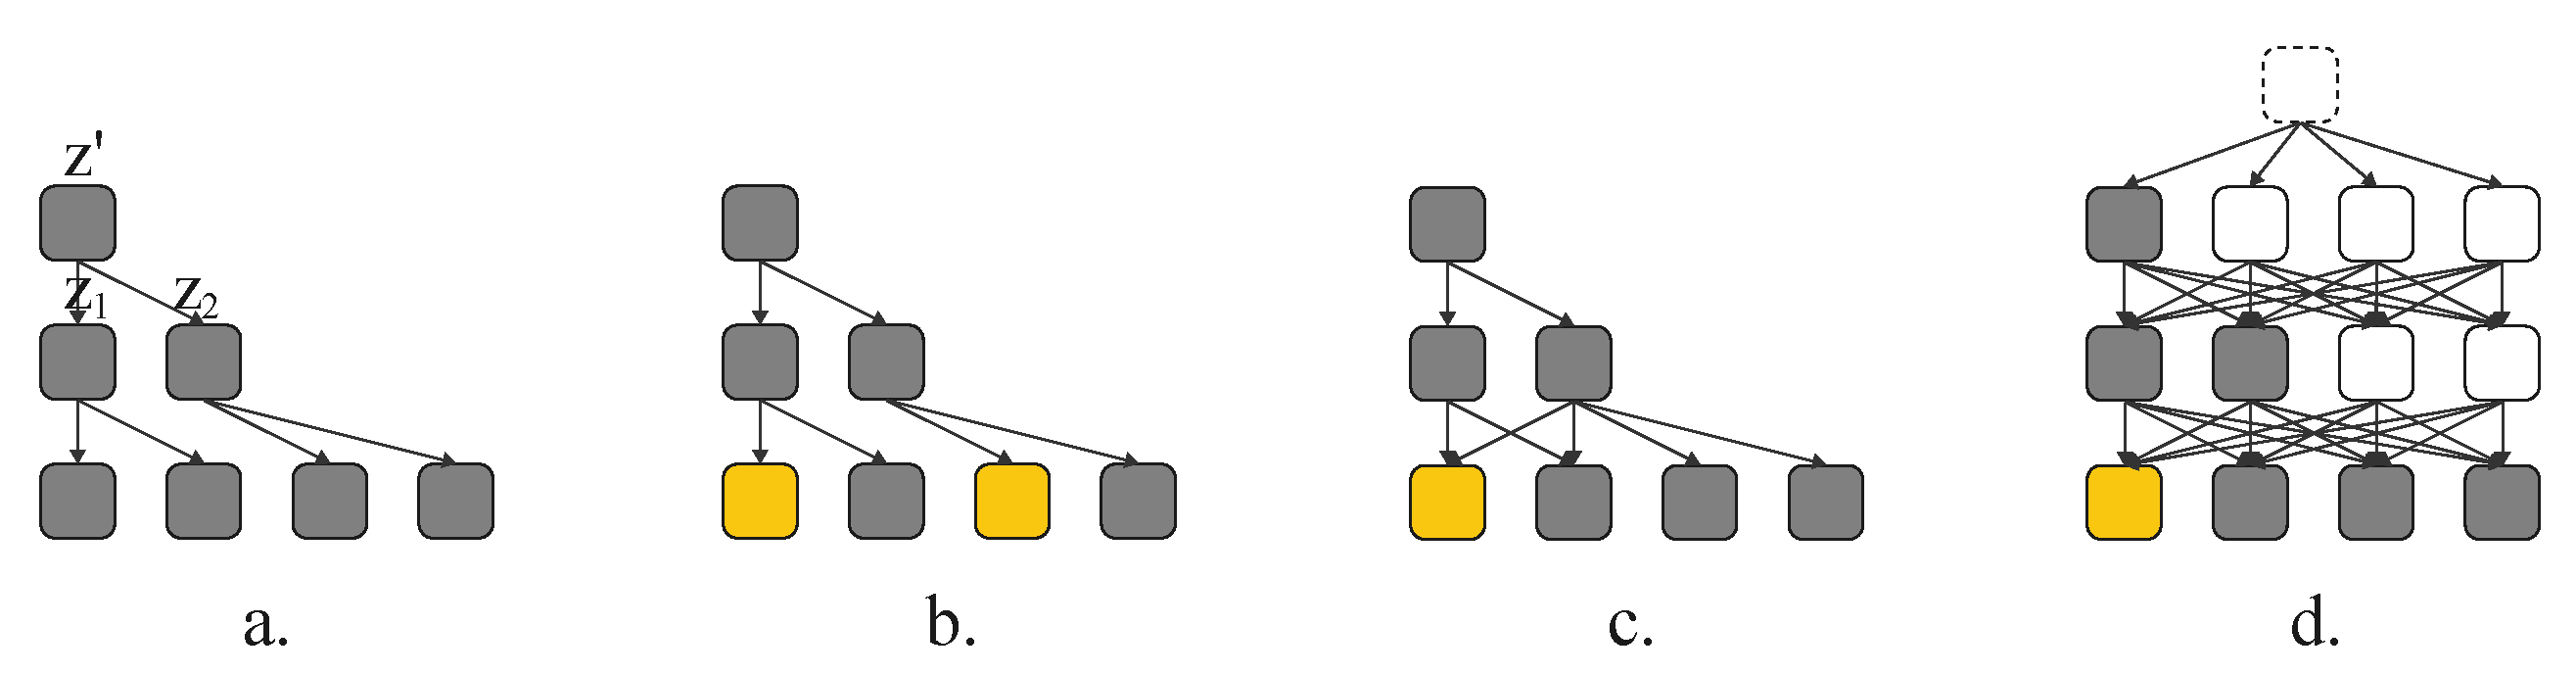
\includegraphics[width=\textwidth]{figures/from-open-universe-to-closed-universe.pdf}
    \caption{One grey box in this figure corresponds to the grey box in figure~\ref{fig:factor-graph-for-inductive-transformer} (a.) Open Universe Model: Every child node has a single parent node.  Parents make categorical choices over existing children.  A child that is activated has only one parent activating it. (b.) Open Universe Model: If two parent nodes would like to activate the same child, we must make a copy of that child.  The two yellow rectangles represent the same concept.  The open universe model must duplicate it in order to allow two parents to utilize it.  (c.) Closed Universe Model: Duplicate concepts are merged into a single node.  A child, therefore, can have more than one parent node.  Since we do not have a potentially infinite layer width, this allows for re-use of limited closed universe resources, and allows for use of scalable closed-universe solvers such as back-propagation.  To do the math correctly when a single child is simultaneously selected by more than one parent, we must use a conditional distribution where if one or more parents selects the child, then the child is activated. (d.) Closed Universe Model: We can make every layer the same width in order to allow for more routes through the model to explain away the data.  This is equivalent to an open universe grammar with N children under the root, and then only N different types of grandchild node, and so forth.}
    \label{fig-appendix:from-open-universe-to-closed-universe}
\end{figure}

\begin{table}[H]
    \setlength{\extrarowheight}{5pt}
    \centering
    \begin{tabular}{c|c|c|c}
        \hline\hline
        child & $\text{parent}_0$ & $\text{parent}_1$ & $p(\text{parent}_0|\text{child}, \text{parent}_1)$ \\[1ex]
        \hline
        1    & 1          & 0          & 1 \\
        1    & 0          & 1          & 1 \\
        1    & 1          & 1          & 1 \\
        0    & 0          & 0          & 1 \\
        1    & 0          & 0          & 0 \\[1ex]
        \hline
    \end{tabular}
    \caption{This table represents the probabilities for some example states of an Open-Closed-Universe factor with two parents and one child.  More details are provided in appendix \ref{appendix:Open-Closed-Universe}}
    \label{tab:open-universe-encoder}
\end{table}

Consider the \emph{decoder},

\begin{equation}
    p(\text{child}) = \sum_{\text{parent}_0} \sum_{\text{parent}_1} 
    p(\text{child}| \text{parent}_0, \text{parent}_1 ) p(\text{parent}_0)p(\text{parent}_1),
\end{equation}

Given table \ref{tab:open-universe-encoder} this marginalization becomes,
\begin{align}
    p(\text{child}=0) &= p(\text{parent}_0=0)p(\text{parent}_1=0) \\
    p(\text{child}=1) &= p(\text{parent}_0=1)p(\text{parent}_1=1) 
    +  p(\text{parent}_0=0)p(\text{parent}_1=1) \nonumber \\
    &\quad+ p(\text{parent}_0=1)p(\text{parent}_1=0),
\end{align}
where we will need to normalize the $p(\text{child})$.  In appendix \ref{fig-appendix:from-open-universe-to-closed-universe} we generalize to arbitrary layer width and provide more exposition.

\subsection{2. Open Closed Universe: Representing an open universe non-parametric model in a closed universe neural network with fixed layer width}\label{appendix:Open-Closed-Universe}

An open universe model does not have fixed layer width. It can sample new branches and nodes into existence when they are needed in order to explain away the data with greater likelihood.  In a ``closed universe'' the network has fixed width and depth.  When we use back-propagation as the solver in such models, it optimizes the weights between existing nodes but it does not create new nodes nor new edges.  Therefore a parent node cannot gain new children, we can only increase the weight between the parent and preexisting child nodes.  In principle we might think that there is no real difference between creating a new node and connecting to an existing node that has not yet been utilized.  But in practice, the form of the activation function of the child node must be adjusted to allow for having multiple parents.

\begin{figure}[H]
    \centering
    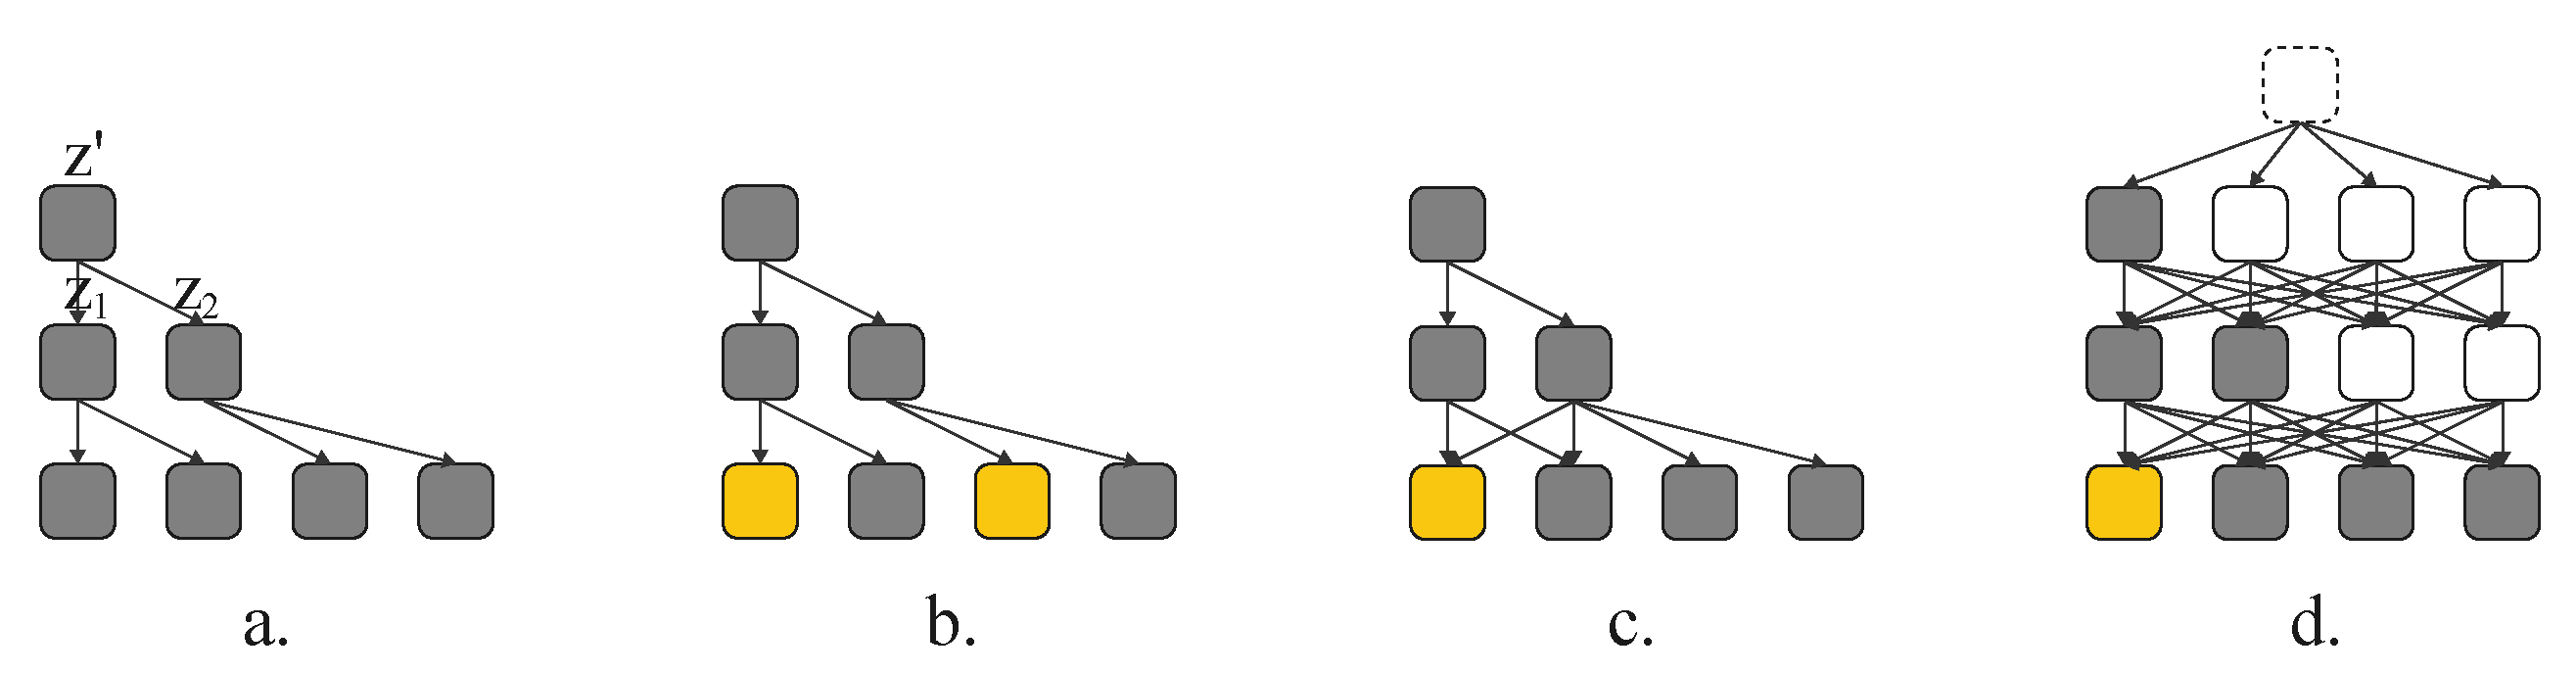
\includegraphics[width=\textwidth]{figures/from-open-universe-to-closed-universe.pdf}
    \caption{Figure provided again for convenience. Again, one grey box in this figure corresponds to the grey box in figure~\ref{fig-appendix:factor-graph-for-inductive-transformer} (a.) Open Universe Model: Every child node has a single parent node.  Parents make categorical choices over existing children.  A child that is activated has only one parent activating it. (b.) Open Universe Model: If two parent nodes would like to activate the same child, we must make a copy of that child.  The two yellow rectangles represent the same concept.  The open universe model must duplicate it in order to allow two parents to utilize it.  (c.) Closed Universe Model: Duplicate concepts are merged into a single node.  A child, therefore, can have more than one parent node.  Since we do not have a potentially infinite layer width, this allows for re-use of limited closed universe resources, and allows for use of scalable closed-universe solvers such as back-propagation.  To do the math correctly when a single child is simultaneously selected by more than one parent, we must use a conditional distribution where if one or more parents selects the child, then the child is activated. (d.) Closed Universe Model: We can make every layer the same width in order to allow for more routes through the model to explain away the data.  This is equivalent to an open universe grammar with N children under the root, and then only N different types of grandchild node, and so forth.}
    \label{fig:from-open-universe-to-closed-universe-appendix}
\end{figure}

\begin{table}[H]
    \setlength{\extrarowheight}{5pt}
    \centering
    \begin{tabular}{c|c|c|c}
        \hline\hline
        child & $\text{parent}_0$ & $\text{parent}_1$ & $p(\text{parent}_0|\text{child}, \text{parent}_1)$ \\[1ex]
        \hline
        1    & 1          & 0          & 1 \\
        1    & 0          & 1          & 1 \\
        1    & 1          & 1          & 1 \\
        0    & 0          & 0          & 1 \\
        1    & 0          & 0          & 0 \\[1ex]
        \hline
    \end{tabular}
    \caption{This table represents unnormalized probabilities for some example states of an Open-Closed-Universe factor with two parents and one child. In the decoder, we will need the conditional probability of the child given all of the parents, $p(\text{child}|\text{parent}_0, \text{parent}_1)$.  In the encoder, we will need the conditional probability of one of the parents, given the child and the other parents, $p(\text{parent}_0|\text{child}, \text{parent}_1)$.  Both conditional distributions can be derived from this same table. In an open-universe model there would be two copies of the child, so that each parent has its own unique children, and therefore each child would have only one parent. When we combine multiple children into a single node with multiple parents, then that combined child should be active if one or more of its parents are active.  This is what we do when we represent an open universe within a closed universe model.  We represent allowed states with a probability of $1$. In this table $\text{probability}=1$ states have the $\text{child}=1$ when any of its parents are a $1$. Another valid state is to have the $\text{child}=0$ when all parents are zeros. Disallowed states (rows) violate those rules and involve one or more parents being a $1$ while the $\text{child}=0$.  Disallowed states have a probability of $0$.}
    \label{tab:open-universe-encoder-appendix}
\end{table}

It is easiest to first consider the \emph{decoder} open-closed-universe-connector where we marginalize for the child given the parents.  We assume all distributions are Bernoulli,

\begin{equation}
    p(\text{child}) = \sum_{\text{parent}_0} \sum_{\text{parent}_1} 
    p(\text{child}| \text{parent}_0, \text{parent}_1 ) p(\text{parent}_0)p(\text{parent}_1),
\end{equation}

where

\begin{equation}
    p(\text{child}| \text{parent}_0, \text{parent}_1) = \begin{cases}
        1 \text{ when } \sum_i \text{parent}_i \geq 1\\
        0 \text{ when } \sum_ i \text{parent}_i = 0.
    \end{cases}
\end{equation}

We often refer to the result on the left hand side of this equation as a ``message''.  A message is the output being computed by a marginalization operation.  An outgoing message in the decoder, we multiply the conditional probability derived from this table by incoming messages $p(\text{parent}_0)$ and $p(\text{parent}_1)$. The message is therefore,

\begin{eqnarray}
    p(\text{child}=0) &=\quad p(\text{parent}_0=0)p(\text{parent}_1=0) \nonumber \\
    p(\text{child}=1)
    &=\quad p(\text{parent}_0=1)p(\text{parent}_1=1) \nonumber \\
    &\qquad+\  p(\text{parent}_0=0)p(\text{parent}_1=1) \nonumber \\
    &\qquad+\  p(\text{parent}_0=1)p(\text{parent}_1=0).
\end{eqnarray}

Finally, we will normalize the outgoing message so that $p(\text{child}=1) + p(\text{child}=0) =1$.

The \emph{encoder} closed-to-open universe factor computes,

\begin{equation}
    p(\text{parent}_0) = \sum_{\text{child}} \sum_{\text{parent}_1} 
    p(\text{parent}_0|\text{child}, \text{parent}_1 ) p(\text{child})p(\text{parent}_1)
\end{equation}

and, 
\begin{equation}
    p(\text{parent}_1) = \sum_{\text{child}} \sum_{\text{parent}_0} 
    p(\text{parent}_1|\text{child}, \text{parent}_0 ) p(\text{child})p(\text{parent}_0)
\end{equation}

Table~\ref{tab:open-universe-encoder-appendix} also defines the distribution $p(\text{parent}_0|\text{child}, \text{parent}_1)$ yielding,

\begin{align}
    p(\text{parent}_0 = 1) &=  
    p(\text{child}=1)p(\text{parent}_1=0) \nonumber \\
    &\quad+ p(\text{child}=1)p(\text{parent}_1=1)\nonumber \\
    p(\text{parent}_0 = 0) &=  
    p(\text{child}=1)p(\text{parent}_1=1) \nonumber \\
    &\quad+ p(\text{child}=0)p(\text{parent}_1=0).
\end{align}

For an arbitrary layer width we have,

\begin{align}
    p(\text{parent}_i = 1) &=  
    p(\text{child}=1) \sum_{j\neq i} \left( p(\text{parent}_j=0) + p(\text{parent}_j=1) \right)
\end{align}


\subsection{Bernoulli-Categorical}\label{appendix:Bernoulli-Categorical}

Consider the conditional distribution $p(y_{\text{Categorical}}=i|y^j_{\text{Ber}}=1, y^k_{\text{Ber}}=0)$ where $j=\text{dog}$ and $k=\text{cat}$, and $i$ varies over the states dog and cat. This is represented in table~\ref{tab:Bernoulli-categorical}.

\begin{table}[H]
    \setlength{\extrarowheight}{5pt}
    \centering
    \begin{tabular}{c|c|c|c}
        \hline\hline
        \textbf{$y_{\textbf{Categorical}}$} & \textbf{$y^{\textbf{dog}}_{\textbf{Ber}}$} & \textbf{$y^{\textbf{cat}}_{\textbf{Ber}}$} & \textbf{probability} \\[1ex]
        \hline
        dog    & 1          & 0          & 1 \\
        cat    & 0          & 1          & 1 \\
        dog    & 1          & 1          & 0 \\
        dog    & 0          & 0          & 0 \\[1ex]
        \hline
    \end{tabular}
    \caption{Each row in this table represents the probability of a joint state for a Categorical and two Bernoullis. In this example, the state of the Categorical can be either dog or cat. One Bernoulli is providing information about if there is a dog or not.  A second Bernoulli tells us if we see a cat or not.  The conditional distribution of the Categorical given both Bernoullis is $p(y_{\text{Categorical}} \in \{\text{dog, cat}\}|y^\text{dog}_{\text{Ber}} \in \{0,1\}, y^\text{cat}_{\text{Ber}}) \in \{0,1\})$.  When the incoming dog-Bernoulli is a 1 and the incoming cat-Bernoulli is a 0, and the categorical is set to its dog state, then this joint state is allowed.  We write the probability for this first row in the table as a 1, knowing that we will ultimately normalize the probabilities across all of the rows.  Similarly we have a probability=1 in the second row where the cat-Bernoulli is 1, the dog-Bernoulli is 0, and the categorical is set to the cat state.  However, as we see in rows 2 and 3, when the dog-Bernoulli and the cat-Bernoulli are both ones or both zeros, these are zero probability joint states.  The Bernoulli-categorical factor obeys the constraint that dog and cat can't both be 1, nor can they both be 0.  Therefore the probabilities in the last two rows are 0.}
    \label{tab:Bernoulli-categorical}
\end{table}

\begin{equation}
    p(y_{\text{Categorical}}=i|y^j_{\text{Ber}}=1, y^k_{\text{Ber}}=0) = \begin{cases}1, \text{ if } i=j \text{ and } i \neq k \\ 0, \text{ otherwise} \end{cases},
\end{equation}

\begin{eqnarray}\label{eq:Bernoulli-categorical}
    p(y_\text{Categorical}=\text{dog}) &=& p(y^\text{dog}_{\text{Ber}}=1)p(y^\text{cat}_{\text{Ber}}=0) \nonumber \\
    p(y_\text{Categorical}=\text{cat}) &=& p(y^\text{dog}_{\text{Ber}}=0)p(y^\text{cat}_{\text{Ber}}=1) 
\end{eqnarray}

Finally we normalize the outgoing message, dividing by $norm=p(y_\text{Categorical}=\text{dog})+p(y_\text{Categorical}=\text{cat})$.

The above can be further simplified.  We illustrate this more clearly in an example with three states, $\{$dog, cat, bird$\}$.

\begin{eqnarray}
    p(\text{dog})& =& p_{\text{dog}}(1)p_{\text{cat}}(0)p_{\text{bird}}(0) \nonumber \\
    p(\text{cat})& =& p_{\text{dog}}(0)p_{\text{cat}}(1)p_{\text{bird}}(0) \nonumber \\
    p(\text{bird})& =& p_{\text{dog}}(0)p_{\text{cat}}(0)p_{\text{bird}}(1)
\end{eqnarray}

Using the fact that $p_{\text{dog}}(0) = 1- p_{\text{dog}}(1)$ we can rewrite $p(\text{dog})$ as,

\begin{eqnarray}
    p(\text{dog}) &=& (1-p_{\text{dog}}(0))p_{\text{cat}}(0)p_{\text{bird}}(0)  \\
    p(\text{dog}) &=& p_{\text{cat}}(0)p_{\text{bird}}(0) - p_{\text{dog}}(0)p_{\text{cat}}(0)p_{\text{bird}}(0).
\end{eqnarray}

We could rewrite $p(\text{cat})$ and $p(\text{bird})$ similarly.  Since we will normalize the Categorical at the end, we can divide $p(\text{dog})$, $p(\text{cat})$ and $p(\text{bird})$ by the same constant at any time during the derivation.  We now choose to divide by $p_{\text{dog}}(0)p_{\text{cat}}(0)p_{\text{bird}}(0)$, which yields

\begin{eqnarray}
    p(\text{dog}) &=& \frac{1}{p_{\text{dog}}(0)} - 1 = \frac{p_{\text{dog}}(1)}{p_{\text{dog}}(0)} \nonumber \\
    p(\text{cat}) &=& \frac{1}{p_{\text{cat}}(0)} - 1 = \frac{p_{\text{cat}}(1)}{p_{\text{cat}}(0)} \nonumber \\
    p(\text{bird}) &=& \frac{1}{p_{\text{bird}}(0)} - 1 = \frac{p_{\text{bird}}(1)}{p_{\text{bird}}(0)}
\end{eqnarray}

Again, the last step is to normalize this distribution.



\subsection{Encoder $\pi$}

$\pi_T$ is used as a choice over tokens, $\pi_Z$ as a choice over concepts in the layer below, and $\pi_\rho$ as a choice over positions.

Starting with the joint distribution $p(z_1 \ldots, z_Z, y)$, in the encoder we would like to marginalize to find $p(y)$,

\begin{eqnarray}
    p(y) &=& \sum_{z_1 \in \{0,1\}}\ldots \sum_{z_Z \in \{0,1\}} p(y, z_1, \ldots, z_Z) \nonumber \\
    &=& \sum_{z_1 \in \{0,1\}}\ldots \sum_{z_Z \in \{0,1\}} p(y|z_1, \ldots, z_Z) p(z_1) \ldots p(z_Z)
\end{eqnarray}

\begin{table}[H]
    \setlength{\extrarowheight}{5pt}
    \centering
    \begin{tabular}{c|c|c|c}
        \hline\hline
        $y_{\textbf{categorical}}$ & $\textbf{z}_1$  & $\textbf{z}_2$ & \textbf{probability} \\[1ex]
        \hline
        1    & 1          & 0          & 1 \\
        1    & 0          & 1          & 1 \\
        0    & 1          & 1          & 1 \\
        0    & 0          & 0          & 1 \\
        0    & 0          & 1          & 0 \\
        1    & 1          & 1          & 0 \\[1ex]
        \hline
    \end{tabular}
    \caption{The allowed states in the $\pi_Z$ factor, and two examples of disallowed states. $\pi$ is an ``exactly-one'' constraint that states that $y=1$ if and  only if $\sum_i z_i = 1$.  In other words, only a single $z_i=1$ is allowed for $y$ to be equal to $1$}. 
    \label{tab:X1}
\end{table}

The probability values in table~\ref{tab:X1} can be expressed as 

\begin{equation}
    p(y=1|z_i, \ldots, z_Z) = 
    \begin{cases}
        1 \text{ when } \sum_{i \in \{1, \ldots, Z\}} z_i = 1 \\
        0 \text{ when } \sum_{i \in \{1, \ldots, Z\}} z_i > 1 \text{ or when }  \sum_{i \in \{1, \ldots, Z\}} z_i = 0.
    \end{cases}
\end{equation}


For example, with only two input children $p(y=0)$ and $p(y=1)$ are:
\begin{eqnarray}
    p(y=1) = p(z_1 = 1)p(z_2=0) + p(z_1 = 0)p(z_2=1) \nonumber \\
    p(y=0) = p(z_1 = 0)p(z_2=0) + p(z_1 = 1)p(z_2=1)
\end{eqnarray}

The $\pi$ where the $z_i$ are Bernoullis is $O(2^Z)$ in $Z$, the number of $z_i$'s.  We will find, however, that if we treat the $z_i$'s as states of a single categorical rather than as independent Bernoullis, the computational complexity simplifies significantly to $O(Z)$.  Let's redo the derivation above but with $z_i$ treated as states of a single Categorical, rather than as multiple Bernoullis.  In order to do this we must treat the entire layer of $\pi$'s jointly. 

In the case of the word or token $\pi_T$, with token vocabulary size $T$ and layer width of size $Z$ indexed by $l$, we have a calculation of complexity $O(Z \cdot T)$,

\begin{eqnarray}
    p(x_l) = \sum_{i \in (1, \dots, T)} \omega_{l,\tau} p(t_\tau)
\end{eqnarray}
where $\omega$'s are learned weights, and $i$ indexes for each token or word. 

In the encoder attention $\pi_Z$, the calculation is $O(Z^2)$,
\begin{eqnarray}
    p(y_k) = \sum_{i \in (1, \dots, Z)} \omega_{ki} p(z_i),
\end{eqnarray}
where in the encoder, $\omega$'s are learned weights and $i$ indexes the $\land$'s in the layer below that are sending their marginalized messages to this encoder $\pi$. 

The token $\pi$ is the same as the attention $\pi$, but instead of connecting to the layer below, it connects directly to the words/tokens in the input data.  In a probabilistic generative grammar this is referred to as a ``terminal'' node. This is in contrast to a non-terminal which generates another layer. In deep learning models, the connection from a terminal node to the data is referred to as a residual or skip connection.

In both cases (token and attention), we normalize over the  output distribution before providing it to the next layer in the network (i.e. the next recursive normalization operation).  We treat the entire layer of $y$ edges as a single distribution, $p(y)$, and normalize,

\begin{eqnarray}
    p'(y_0) = p(y_0)/\sum_k p(y_k) \nonumber \\
    p'(y_1) = p(y_1)/\sum_k p(y_k).
\end{eqnarray}

We do the same for the entire layer of $x$ edges,

\begin{eqnarray}
    p'(x_0) = p(x_0)/\sum_k p(x_k) \nonumber \\
    p'(x_1) = p(x_1)/\sum_k p(x_k).
\end{eqnarray}

In summary, compared to the Bernoulli version that we derived first, it makes sense to use this categorical version of $\pi$, because it simplifies the computational complexity from $O(2^n)$ to $O(n^2)$.  Furthermore, in the decoder if we used a Bernoulli version, when computing a particular $p(z_i)$ for exact forward-backward marginalization we would be required to utilize the backward messages for $p(z_{j \neq i})$.  With $p(z)$ being a single joint variable however, there are two incident edges to a decoder $\pi$, $p(x)$ and $p(z)$.  This means when computing a message $p(z)$ in the decoder, we only need the decoder message $p(x)$.  We do not need any messages provided from the encoder.


\subsection{Categorical-To-Bernoulli}\label{appendix:Categorical-To-Bernoulli}

\begin{figure}[H]
    \centering
    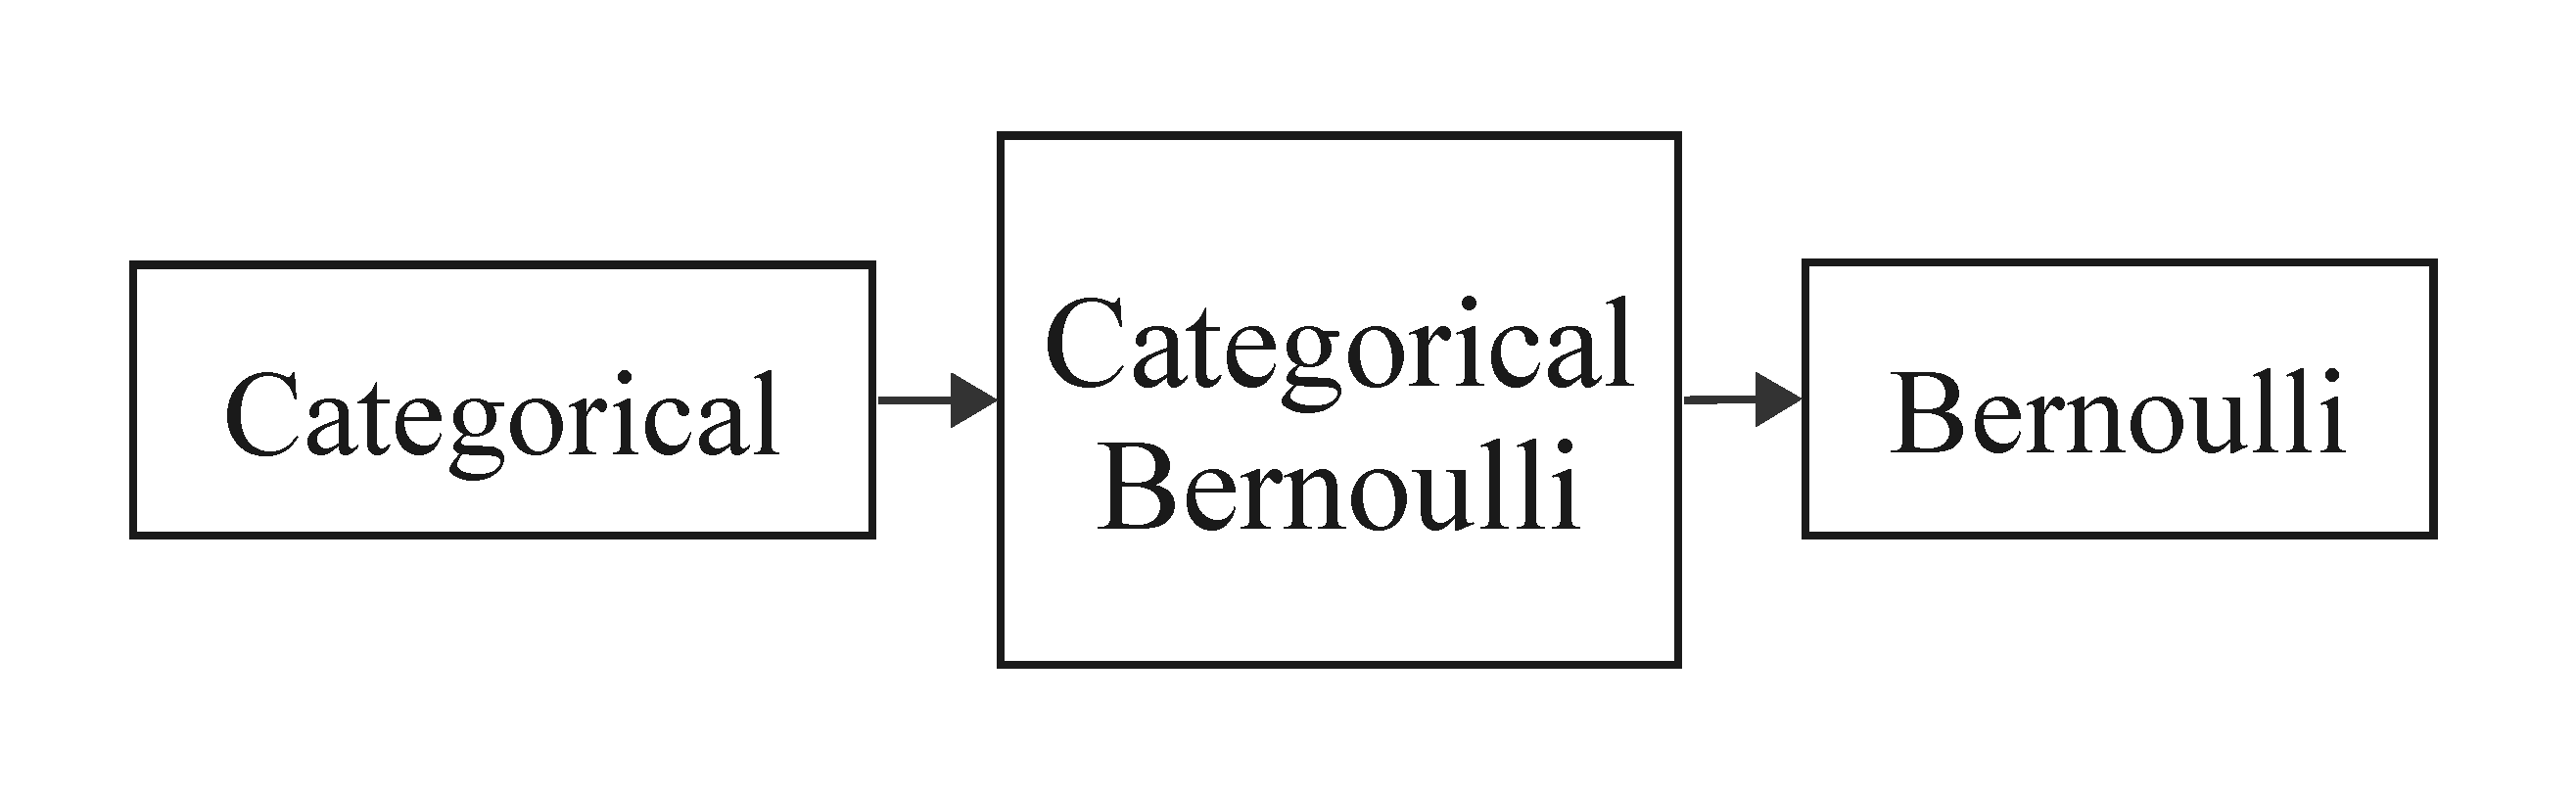
\includegraphics[scale=0.15]{figures/categorical-bernoulli.pdf}
    \caption{Factor Graph for Categorical to Bernoullis Factor}
    \label{fig:categorical-to-bernoulli-single}
\end{figure}


Let us start with an example with only one Bernoulli (a dog-Bernoulli $\in \{0,1\}$) and one Categorical (with states $\in \{\text{dog, cat}\}$, see figure~\ref{fig:categorical-to-bernoulli-single}).  

\begin{align}
    p(z^\text{dog}_{\text{Ber}}=1)
    &= \sum_{z_\text{Categorical} \in \text{dog, cat}} p(z^\text{dog}_{\text{Ber}}=1, z_{\text{Categorical}}) \nonumber \\[5pt]
    &= \sum_{z_\text{Categorical} \in \text{dog, cat}} p(z^\text{dog}_{\text{Ber}}=1|z_{\text{Categorical}})p(z_{\text{Categorical}}) \nonumber \\[7pt]
    &= p(z^\text{dog}_{\text{Ber}}=1|z_{\text{Categorical}}=\text{dog})p(z_{\text{Categorical}}=\text{dog}) \\
    &\quad+ p(z^\text{dog}_{\text{Ber}}=1|z_{\text{Categorical}}=\text{cat})p(z_{\text{Categorical}}=\text{cat}) \nonumber \\[5pt]
    &= 1 \cdot p(z_{\text{Categorical}}=\text{dog}) + 0 \cdot p(z_{\text{Categorical}}=\text{cat}) \nonumber \\[5pt]
    &= p(z_{\text{Categorical}}=\text{dog}) \\[7pt]
    p(z^\text{dog}_{\text{Ber}}=0)
    &= p(z^\text{dog}_{\text{Ber}}=0|z_{\text{Categorical}}=\text{dog})p(z_{\text{Categorical}}=\text{dog}) \\
    &\quad+ p(z^\text{dog}_{\text{Ber}}=0|z_{\text{Categorical}}=\text{cat})p(z_{\text{Categorical}}=\text{cat}) \nonumber \\[5pt]
    &= p(z_{\text{Categorical}}=\text{cat}).
\end{align}


The Bernoulli and the categorical in this example are really saying the same thing. The mutually exclusive alternative to a dog in the Categorical is a cat.  The mutually exclusive alternative to a 1 for the dog-Bernoulli is a 0.  The probability of cat in the Categorical should be equal to the probability of a 0 in the Bernoulli.

Now let's introduce an explicit cat-Bernoulli into the example.

\begin{figure}[H]
    \centering
    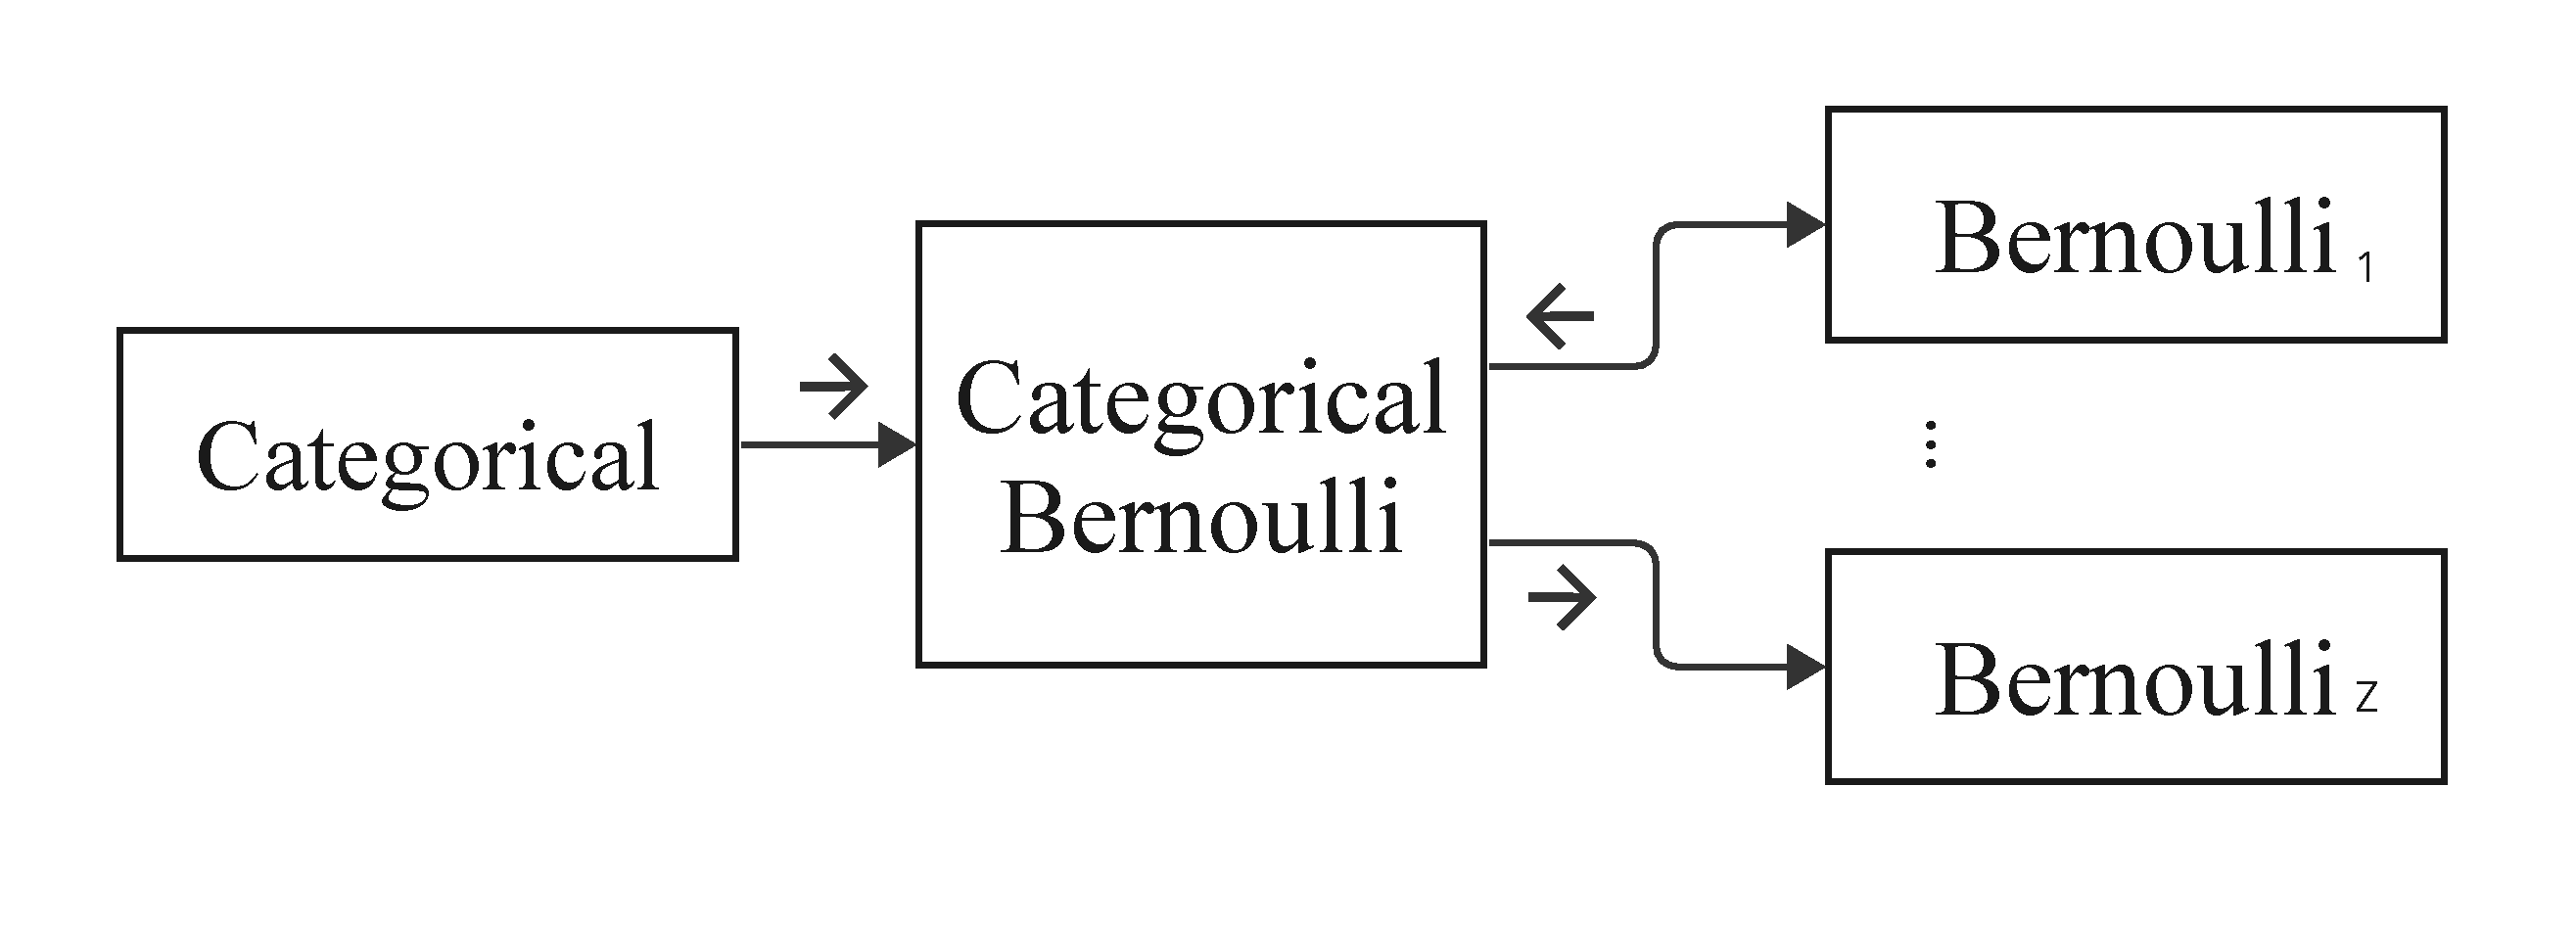
\includegraphics[scale=0.15]{figures/categorical-bernoulli-message-directions.pdf}
    \caption{Factor Graph for Categorical to Bernoulli Factor.  The arrows indicate the direction of the messages.}
    \label{fig:categorical-to-bernoullis}
\end{figure}

Recall that the rule for marginalization within a factor graph is that we compute an outgoing message from a factor using the incoming messages on all other edges incident to the factor.  This is not important in the encoder when we are still doing a forward marginalization pass and there is no useful backward information available yet.  We must consider it, however, in the decoder if we wish to do full forward-backward marginalization. % That said, we will ultimately choose to do forward-only marginalization~\ref{appendix:connectivity}.

As we can see in figure~\ref{fig:categorical-to-bernoullis}, when we add a Bernoulli for cat, and compute an outgoing message for the dog-Bernoulli, we also need an incoming message from the cat-Bernoulli.

We recall table~\ref{tab:Bernoulli-categorical}, but move the columns around to fit our current situation.  Again, each row represents the probability of a joint state when we have two Bernoullis (dog and cat) and one Categorical with two states (also dog and cat).

\begin{table}[H]
    \setlength{\extrarowheight}{5pt}
    \centering
    \begin{tabular}{c|c|c|c}
        \hline\hline
        \textbf{$z^{\textbf{dog}}_{\textbf{Ber}}$} & \textbf{$z_{\textbf{Categorical}}$} & \textbf{$z^{\textbf{cat}}_{\textbf{Ber}}$} & \textbf{probability} \\[1ex]
        \hline
        1          & dog    & 0          & 1 \\
        0          & cat    & 1          & 1 \\
        1          & dog    & 1          & 0 \\
        0          & dog    & 0          & 0 \\[1ex]
        \hline
    \end{tabular}
    \caption{}
    \label{tab:categorical-bernoulli}
\end{table}

We care about computing the marginal probability for a given Bernoulli, e.g. $p^{\text{dog}}_{\text{Ber}}(1)$,

\begin{align}
    p^{\text{dog}}_{\text{Ber}}(1) 
    &= \sum_{z_{\text{Categorical}}} \sum_{z^{\text{cat}}_{\text{Ber}}} p(z^{\text{dog}}_{\text{Ber}}, z^{\text{cat}}_{\text{Ber}}, z_{\text{Categorical}}) 
    \nonumber \\
    &= 
    \sum_{z_{\text{Categorical}}} \sum_{z^{\text{cat}}_{\text{Ber}}} 
    p(z^{\text{dog}}_{\text{Ber}}| z^{\text{cat}}_{\text{Ber}}, z_{\text{Categorical}})p(z^{\text{cat}}_{\text{Ber}})
    p(z_{\text{Categorical}}).
\end{align}

For this calculation, we need the conditional probability $p(z^{\text{dog}}_{\text{Ber}}=1 | \ldots)$,  

\begin{align}
        p(z^{\textrm{dog}}_{\text{Ber}}=1|z_{\text{Categorical}}=j, z^{\text{cat}}_{\text{Ber}}) 
        &= \begin{cases}
        1, \text{ when } z_{\text{Categorical}}=\text{dog}, z^{\text{cat}}_{\text{Ber}}=0 \\ 
        0, \text{ otherwise }  
        \end{cases}.
\end{align}

We can write this more generally, with $i$ instead of ``dog'' and $j$ for the state of $z_\text{Categorical} = j$, and with $Z$ Bernoulli variables indexed by $k$,

\begin{align}
        p(z^{i}_{\text{Ber}}=1|z_{\text{Categorical}}=j, z^1_{\text{Ber}}, \ldots, z^{i-1}_{\text{Ber}}, z^{i+1}_{\text{Ber}}, \ldots, z^Z_{\text{Ber}}) \\=
        \begin{cases}
        1 \text{ when } j=i, \text{ and } z^k_{\text{Ber}}=0 \ \forall k \neq i \\ 
        0, \text{ otherwise }  
        \end{cases}.
\end{align}

To compute the marginal probability $p^{\text{dog}}_{\text{Ber}}(0)$, we will need the conditional probability $p(z^{\text{dog}}_{\text{Ber}}=0 | \ldots)$.  This conditional probability is a $1$ when $z^{\text{cat}}_{\text{Ber}}=1$ and $z_{\text{Categorical}} =\text{cat}$.  In other words, we need an allowed state with $z^{\text{dog}}_{\text{Ber}}=0$, which means that overall we need a joint ``cat'' state.  

More generally, if we have more Bernoullis, we need to allow joint states for ``bird'' or other allowed states, $j$.  An allowed state always has $z_{\text{Categorical}} = j$ and also has $z^j_{\text{Ber}}=1$ and all other Bernoullis $z^{i \neq  j}_{\text{Ber}}=0$.  Therefore the $\sum_i z^{i}_{\text{Ber}}=1$.  Putting this all together we write,

\begin{align}
        p(z^{i}_{\text{Ber}}=0|z_{\text{Categorical}}=j, z^1_{\text{Ber}}, \ldots, z^{k-1}_{\text{Ber}},z^{k=j}_{\text{Ber}}, z^{k+1}_{\text{Ber}}, \ldots, z^Z_{\text{Ber}}) 
        \\= 
        \begin{cases}
        1 \text{ when } \sum_{k} z^{k}_{\text{Ber}}=1 \text{ and } j \neq i\\
        0 \text{ otherwise }
        \end{cases}.
\end{align}

The computation for $p(z^{i}_{\text{Ber}}=0)$ will contain only one product per Bernoulli.  So the computations involving incoming Bernoulli messages are not prohibitively complex. We might not need to do them at all, however.  In the encoder we use a categorical-Bernoulli as we send forward messages from the $\pi$ to the $\land$, but in the encoder there is not yet any backward information to incorporate into our calculation.

Then in the decoder, we convert from categorical-Bernoulli as we send marginals from the $\pi$ to the open universe.  We could, however, simply choose to ignore the forward messages from the encoder.  This approximation to exact marginalization is further discussed in section~\ref{appendix:decoder-and}.

In summary, the Categorical-to-Bernoulli gets used in two places.  In the encoder, where we will ignore backward messages because they do not yet carry any information, and in the decoder where we can choose to ignore forward messages. If in the decoder, we ignore the forward messages from the encoder, then how do the encoder and decoder differ?  The answer is that the encoder turns tokens into a deep ``concept'' representation, while the decoder then uses layers of ``concepts'' to generate tokens.

If, when calculating an outgoing Bernoulli message, we do not need to use the other incoming Bernoulli messages then we can simplify our computation considerably.  We can set them to be non-informative (e.g. $p(z_{\text{Ber}})=0.5$).  Let us do a pedagogical example with a categorical and three Bernoullis representing ``dog'', ``cat'', and ``bird''.

\begin{align}
    p({z^{\text{dog}}_{\text{Ber}}}=1) 
    &= 
    p(z_{\text{Categorical}}=\text{dog})
    p({z^{\text{cat}}_{\text{Ber}}}=0)
    p({z^{\text{bird}}_{\text{Ber}}}=0), \\
    p({z^{\text{dog}}_{\text{Ber}}}=0)
    &= p(z_{\text{Categorical}}=\text{cat})
    p({z^{\text{cat}}_{\text{Ber}}}=1)
    p({z^{\text{bird}}_{\text{Ber}}}=0), \nonumber \\
    &\quad+ p(z_{\text{Categorical}}=\text{bird})
    p({z^{\text{cat}}_{\text{Ber}}}=0)
    p({z^{\text{bird}}_{\text{Ber}}}=1)
\end{align}\\

Now if $p({z^{\text{bird}}_{\text{Ber}}}=1) = p({z^{\text{bird}}_{\text{Ber}}}=0) = p({z^{\text{cat}}_{\text{Ber}}}=1) = p({z^{\text{cat}}_{\text{Ber}}}=0) = 0.5$ then,\\
\begin{align}
    p({z^{\text{dog}}_{\text{Ber}}}=1) 
    &= 
    p(z_{\text{Categorical}}=\text{dog})(0.25), \\
    p({z^{\text{dog}}_{\text{Ber}}}=0)
    &= p(z_{\text{Categorical}}=\text{cat})(0.25) + p(z_{\text{Categorical}}=\text{bird})(0.25)
\end{align}

More generally, after normalizing this becomes,

\begin{align}
    p(z^i_{\text{Ber}}=1) &= p(z_{\text{Categorical}}=i) \nonumber \\
    p(z^i_{\text{Ber}}=0) &= \sum_{j\neq i} p(z_{\text{Categorical}} =j)
\end{align}


\subsection{Encoder $\land$}


The encoder $\land$ is a constraint that imposes z = AND(x,y) as shown in the truth table below.  The (four) allowed states have non-zero probabilities normalized to $1/4$. The dis-allowed states have zero probability.

\begin{table}[H]
    \setlength{\extrarowheight}{5pt}
    \centering
    \begin{tabular}{c|c|c|c}
        \hline\hline
        x & y & z & probability \\[1ex]
        \hline
        0    & 0   & 0          & 1/4 \\
        0    & 0   & 1          & 0 \\
        0    & 1   & 1          & 1/4 \\
        0    & 1   & 1          & 0 \\
        1    & 0   & 0          & 1/4 \\
        1    & 0   & 1          & 0 \\
        1    & 1   & 0          & 0 \\
        1    & 1   & 1          & 1/4 \\[1ex]
        \hline
    \end{tabular}
    \label{tab:open-universe-encoder-truth-table}
\end{table}

One way to think about these modules is to imagine that $x$ is a stochastic stream of 0's and 1's, where the 1's occur with probability $p_x$ and 0's with probability $1-p_x$.  Similarly, imagine $y$ as a stochastic stream of 0's and 1's, where the 1's occur with probability $p_y$ and 0's with probability $1-p_y$.  When we marginalize to find $p(z)$ we are answering the question, ``if the stochastic streams for $x$ and $y$ passed through a logical AND gate, what would be the percentage of 1's and 0's in the output stream for $z$?''

We answer this question by computing the marginal probability for $p(z)$,

\begin{eqnarray}
    p(z) &=& \sum_{x, y} p(x, y, z) \nonumber \\
     &=& \sum_{x, y} p(z|x, y)p(x)p(y) \nonumber \\
     &=& \sum_{x, y} \delta(z-\land(x, y))p(x)p(y) \nonumber \\
    p(z_l) &=& \sum_{x, y} \delta(z-\land(x_l, y_l))p(x_l)p(y_l)
\end{eqnarray}
where $l$ indexes across a layer of the model. So, in our simple example we have:

\begin{align}\label{eq:encoder-and}
    p(z_l = 1) &= p(x_l=1)p(y_l=1) \nonumber \\
    p(z_l = 0) 
    &= p(x_l = 0)p(y_l=0) \nonumber \\
    &\quad+ p(x_l = 0)p(y_l=1) \nonumber \\
    &\quad+ p(x_l = 1)p(y_l=0).
\end{align}


\subsection{Decoder $\land$}\label{appendix:decoder-and}

The decoder $\land$ is very similar to the encoder $\land$,

\begin{eqnarray}\label{eq:decoder-and}
    p_{\text{y decode}}(1) &= p_{\text{x encode}}(0)p_{\text{z decode}}(0) + p_{\text{x encode}}(1)p_{\text{z decode}}(1) \nonumber \\
    p_{\text{y decode}}(0) &= p_{\text{x encode}}(0)p_{\text{z decode}}(0) + p_{\text{x encode}}(1)p_{\text{z decode}}(0) 
\end{eqnarray}

As we can see, when the decoder $\land$ is computing $p_{\text{decode}}(y)$, it should not only use $p_{\text{decode}}(z)$, it should also use $p_{\text{encode}}(x)$.
Similarly, when the decoder $\land$ is computing $p_{\text{decode}}(x)$, marginalization should use $p_{\text{encode}}(y)$.  However, this would mean that to predict $p_{\text{decode}}(x)$ at a given position, the model is using information from tokens to the right in the text.  Indeed, not using $p_{\text{encode}}(y)$ in the decoder is the equivalent of forward-only message passing in belief propagation~\citep{BenVigodaThesis, murphy2002dynamic} which predicts the next symbol in a sequence based only on previous signals. Thus, we could choose not to use  $p_{\text{encode}}(x)$ and $p_{\text{encode}}(y)$ in the decoder to train it for this task.

The next layer in the decoder is the Bernoulli-Categorical, which we have already described above.  Next we describe the decoder $\pi_T$.

\subsection{Decoder Token $\pi$}

Let us consider a single $\pi$ within a layer of the model. $p(x)$ is an output of the decoder $\land$ which becomes the input to this $\pi$. The marginal probability of generating token $t$ from $\pi$ is,

\begin{align}
    p(t=\tau) &= p(t=\tau|x) p(x), \nonumber \\
    p(t=\tau) &= \omega_\tau \cdot p(x),
\end{align}

Sampling from this distribution, we would get a single token with probability $\omega_{t}$, where $\omega$'s are learned weights.

We are treating $p(t)$ as a Categorical with a state for each token, so we might think that we need to normalize such that $\sum_{\tau} p(t_\tau) = 1$.  This would be incorrect.
We do use normalized (learned) weights such that, $\sum_\tau \omega_{\tau} = 1$, but we do not normalize the output of the decoder $\pi$'s.

The reason is that this is another situation where we must take into account the open-closed universe factor.  Each $\pi^l_t$ in the layer indexed by $l$ has some probability outputting a given token, e.g. ``cat''.  These $\pi^l_t$'s share children.  We can see in figure~\ref{fig-appendix:factor-graph-for-inductive-transformer}, that the output of the decoder $\pi_Z$ goes through a Categorical-to-Bernoulli and then into an open-closed universe layer, both as described above in appendices~\ref{appendix:Open-Closed-Universe} and~\ref{appendix:Categorical-To-Bernoulli}.

What we are really doing when we do not normalize the outputs of an individual decoder $\pi$ within a single layer, is allowing the $\pi$'s to each participate proportionally in activating their shared children and have the normalization come out correctly as it would in an open universe.

For example, for a particular $\pi_t$, when the input is p(x=1) = 80\% and p(x=0)=20\%, and the $\pi_t$ weights are dog weight = 50\% and cat weight = 50\%, then the probability of outputting the word dog, p(dog)=40\%, p(cat)=40\% and the (un-normalized) probability of outputting no token at all is p(no output)=20\%.  In this case, we allow some other $\pi_{j \neq i}$ to generate the word.


\section{Self-Attention in the Inductive Transformer}

\subsection{Vanilla Self-Attention}\label{appendix:vanilla-self-attention}

Many variants of the transformer have appeared since the publication of the original ``vanilla'' version, so we should not be overly pedantic as we derive the corresponding inductive transformer attention mechanism.  Our derivation will actually skew more closely to the relative positional encodings formulation of the transformer in Transformer-XL than to the vanilla version~\citep{dai2019transformerxl}. 

Regardless, it is useful to recall that the core of self-attention in a vanilla transformer~\citep{vaswani2017attention} is,\footnote{We suppress chunking which is used for parallel computing in hardware, but is a distraction when describing the model.}  

\begin{align} \label{eq:vanilla-self-attention}
    Y_i &= \sum_j\text{softmax} \Bigg(\frac{Q_i \cdot K_j^T}{\sqrt{d}} \Bigg) V_j,
\end{align}
where $Q$, $K$, and $V$ are the query, key, and value matrices, each formed by applying matrices $W^Q$, $W^K$, $W^V$ to the embedding vector input to this attention layer at each position, and where $d$ is the embedding dimension.  Because of the softmax operation, each row of the $Q_i \cdot K_j^T$ matrix is a normalized set of weights for linearly combining vectors $V_j$.  


\subsection{A Generative Production for Self-Attention}

Now we would like to understand the attention mechanism in terms of a conditional probability distribution $p(y| \ldots)$ over discrete variables.  We stress the point, because if we want to design inductive bias, then this becomes much easier if we can examine the model in isolation from how we will solve it. We therefore want to interpret our ``analog'' activations in the marginalization of the model as expressions of uncertainty about underlying ``digital'' variables.  This reasoning forces us into a stance of modeling the underlying variables and then inferring on representations of their uncertainty or probability.  

Why would we expect a large language model to be estimating uncertainty about discrete variables?  Because these systems are solving an inverse problem.  If you want to guess what concepts I am thinking as I say something to you, so that you can model my concepts and reply appropriately (theory of mind), then the operation I performed which was to transform my concepts into speech must be inverted by you who now must (approximately) convert my speech back into concepts.  Since the mapping from concepts to speech is many-to-many, in listening to me, you have an inherently under-determined problem to solve, which by its nature requires representing the uncertainty of competing interpretations of the data.  That said, presumably I am certain about what I am thinking as I talk about it. In other words there are some underlying, highly certain, discrete variables in my mind that you need to estimate.

It is not at all uncommon in machine learning systems for some operations to occur in the probability domain, some in the log probability domain, and even for a machine learning system to perform operations in a domain that might best be described as a second order Taylor series approximation to the log probability domain.  For example, above-threshold CMOS analog implementations of neural networks and probabilistic models take this approach, since the transfer function of these transistors is $I \propto V^2$~\citep{BenVigodaThesis}. Furthermore, since taking a log is monotonic, and since during training we care mostly about gradients, although the choice of domain may impact numerical stability, it often does not materially impact the expressiveness of the model.

To derive the inductive transformer attention, instead of describing matrix operations on embedding vectors to compute $Y$ as we did in equation~\ref{eq:vanilla-self-attention}, we will first start from $Y$ and describe a sequence of stochastic sampling operations to arrive at values for $v_j$.  Think of these sampling operations as proceeding backwards through the encoder, towards the input text.

We start our generative statistical model by defining $i \in \{1 \ldots P\}$ which we treat as an absolute position index, and $j \in \{1 \ldots P\}$ which we treat as a relative position index:
\begin{enumerate}
    \item $i \sim p(i)$: Given $y$ in the self-attention equation~\ref{eq:vanilla-self-attention}, sample a position $i$ from a categorical distribution, $p(i|y)$.
    \item $j \sim p(j|i)$: Given position $i$, sample a relative position $j$ to attend to. The weight $\omega_{j,i} = p(j|i)$ corresponds to $q_i \cdot k_j$ in the attention matrix (more on this in a moment).  As discussed below, we can add any desired prior to our distribution $p(s)$ as a prior on our attention weights $p(j|i, s)p(s)$ in order to sparsify the weights.
    \item $v \sim p(v|j)$: $p(v|j)$ is the prior on values in an embedding vector.  For simplicity, we start with a categorical distribution.  We discuss how this can be represented as a denser embedding vector in appendix \ref{appendix:from-indicator-to-embedding}.
    \item We leave $W^q$, $W^k$ for later in our discussion.
\end{enumerate}
These steps together form the conditional probability distribution,
\begin{equation}
    p(v|j)p(j|i)p(i|y)p(y). \label{eq:prob-position-generate}
\end{equation}

Regarding $p(s)$, it is now commonplace to design sparse attention patterns to achieve $O(n \log n)$ or $O(n \sqrt{n})$ complexity~\citep{DBLP:journals/corr/abs-2009-06732, DBLP:journals/corr/abs-2007-14062}.  Additionally there are more recent grammatical attention patterns that achieve a sentence-level inductive bias towards grammatical constructions~\citep{sartran2022transformer}. Although certainly useful, these priors on the attention weights are distinct from the additional inductive bias provided by the inductive transformer in the feed-forward layers of the transformer. 

The interesting term is $p(j|i)$.  This corresponds to the vanilla attention matrix.  In vanilla notation, the elements of the attention matrix which depend on inner products of $Q_i$ and $K_j$, where $Q_i = W^q X_j$ and $K_j = W^k X_j$ and where $X_j$ is an embedding vector at position $j$ in the data window. 

\subsection{Inference in the Inductive Transformer Attention Layer}

We use probabilistic notation that corresponds to the vanilla notation so that,

\begin{equation}\label{eq-appendix:encoder-attention}
    p(y) =
    \sum_{q,k}p(y|q,k,v)
    \sum_{x^q, x^k, x^v} p(q|x^q)p(k|x^k)p(v|x^q)
    \sum_x p(x^q, x^k, x^v|x)p(x),
\end{equation}

where $p(y|q,k, v)$ is the attention matrix.  We have represented how the variables in the attention mechanism are connected as a product of conditional distributions.  Leave aside for the moment that these may not be well formed probabilities in the actual implementation of a transformer. Assume as discussed above that they in some sense represent levels of certainty about something.  For now we focus on the factorization of the model.

If we want to turn this distribution around so that we can understand what the underlying production is that samples $p(x)$, or so that we can perform decoder marginalization to find the marginal probability $p(x)$ we might get confused. It might seem like we are going to get circular reasoning where $p(x|v)$ depends on $p(v|y, k, q)$ and $p(k|x)p(x)$ depends on $x$.

The trick is to realize that this is like a situation where we are trying to measure the same underlying quantity three times in three different ways.  In a sense, $p(q|x^q)$, $p(k|x^k)$, and $p(v|x^q)$ are all measurements of an underlying variable $x$ such that $p(x^q, x^k, x^v|x) = \delta(x^q-x)\delta(x^k-x)\delta(x^v-x)$. 

As an example, suppose that we are trying to measure a pillow using three different measuring devices -- a caliper, a yard stick and a tape measure.  The generative model could be, sample the actual length of the pillow from some prior distribution, perhaps a Gaussian with mean 18 inches and variance 4 inches.  Then call a function for each measuring device which takes in the sampled length and outputs a simulated measurement by that device.  For example maybe the yard stick tends to over-estimate the length of the pillow because it squashes and extends the pillow while the tape measure tends to get tangled and vastly over-estimate the length and the caliper tends to under-estimate because it can only open to 16 inches maximum.  Now we have three ways to measure the same thing.  And it is not so strange to think that we might have learned some things in the past about each of these measuring devices.  So, for example, when the yard stick and the tape measure both agree that the object is 3 feet long, we tend to throw away the measurement from the calipers which is way too short to be helpful in those situations.  Similarly, if the yard-stick and the tape measure tell us that the object is less than one inch long, we might primarily use the estimate from the calipers, because it is most accurate for short distances.  This is essentially what the attention matrix is learning to do. 

To compute the decoder marginal $p(x)$ conditioned on $p(q)$ and $p(k)$ is seemingly straight-forward, we simply compute the attention matrix from the inner products of $p(q)$ and $p(k)$, and use each row of the attention matrix as the normalized weights for a categorical distribution which chooses a position in $P$.

We must remember, however, that for example $p(q) = \sum_x p(q|x)p(x)$ where $p(q|x)$ represents our learned posterior about how $q$ measures $x$.  In theory this requires loopy belief propagation that proceeds from $x$ to $q$ and $k$ to form the attention matrix, brings in any information from $p(y)$ and then estimates $p(v|q, k, y)$ and finally marginalizes $p(x|v)p(v)$ to find $p(x)$.  Luckily, as we can see from the equation \ref{eq-appendix:encoder-attention}, loopy inference is not necessary in the encoder marginalization.  

For the decoder marginalization, in practice, we mask the attention so that the decoder cannot attend to future tokens, and we condition the decoder on tokens that have already been generated. This effectively eliminates the loops.  Like any backward marginalization pass in any model, the decoder attention consumes messages from the encoder, namely $q$.

The vanilla decoder uses the same attention mechanism as the encoder attention. For some types of factors, marginalization in each direction is highly asymmetric, but as we saw in our $\pi_Z$ and $\pi_T$ factors, for categorical distributions of the type that appear in the attention mechanism, this distinction is less critical.

There are a range of published variants of the vanilla attention mechanism.  We have attempted to capture the essential properties of most attention mechanisms in the marginalization of this model.  That said, there is no reason why an existing attention mechanism couldn't be incorporated into the inductive transformer with the overall model still benefiting from the additional inductive bias provided in other layers such as the modified feed-forward layer.

\section{$\land$ in the Log Probability Domain}
\label{appendix:log-probability-and}

After the feed-forward layer, the vanilla transformer has an add \& norm layer that adds in the residual connections and normalizes the output of the layer. Our layer of $\land$ activation functions in figure~\ref{fig:factor-graph-for-inductive-transformer} performs the analogous operation in the inductive encoder. Recall, from equation~\ref{eq:encoder-and} that the probability $p(z=1)$ is given by the product of the probabilities $p(x)$ and $p(y)$. In the log domain this results in,
\begin{eqnarray}
    \log p(z=1) = \log p(x=1) + \log p(y=1).
\end{eqnarray}
As we normalize after computing this activation function, this mimics the behavior of the ``Add \& Normalize'' layer in the vanilla transformer.

Note that the vanilla encoder has an additional add \& norm layer after the feed-forward.  We would argue that the sum with residuals here is incorrect, but the layer norm does correspond to the Bernoulli to categorical that happens after the encoder close-open-universe factor. 


\section{From Indicator Vectors to Embedding Vectors}\label{appendix:from-indicator-to-embedding}

Until now we have been assuming embedding vectors that are categorical distributions.  Categorical vectors are not an efficient embedding, but they are easy to understand.  They are of length $T$, the number of tokens in the vocabulary, indexed by $t \in \{1, \ldots, T\}$, or of length $P$ the number of positions in the input data window and indexed by $\rho$.  Each element in these categorical vectors represents $p(t)$, the probability of the $t^\mathrm{th}$ token or $p(\rho)$ the probability of the $\rho^\mathrm{th}$ position.  Just as in the vanilla transformer, categorical embeddings can be used to represent not just tokens but all kinds of information deep within a network.  Throughout this paper we have done just that.  The inner product of two indicator vectors is meaningful as a measure of the distance between two categorical distributions, so we can compute semantic distance just as we would with dense embedding vectors.

As in the vanilla transformer, at the input of the inductive transformer we have an embedding vector for each token position in order to represent the token that is present at that position.  If, as is true at the input to the network, we are certain about what token is present at a given position, then we have a ``one-hot'' vector with a single probability that is $\approx 1$ for the $t^\text{th}$ token and $\approx 0$ elsewhere.  If, as is true at the output of the network, we have a categorical distribution over tokens, then we have an array of probabilities from which we can sample a token.  The inputs and outputs are therefore identical to those of the vanilla transformer.

In order to implement \emph{dense} embedding representations within the inductive transformer, we do the typical thing and use an embedding matrix $E$ to transform a categorical vector to a lower dimensional embedding vector,

\begin{align}
    p(i_{\text{embedding}}) 
    &= E \cdot p(i_{\text{categorical}}) \\
    &= \sum_{i_{\text{categorical}}} p(i_{\text{embedding}}|i_{\text{categorical}})
    p(i_{\text{categorical}}),
\end{align}

and then at the output use $E^T$ to transform from an embedding vector back to a categorical vector.  The only problem with this approach for the inductive transformer is that all of our factors were defined to operate on categorical variables and/or to transform a categorical variable to a group of Bernoulli variables, operate on Bernoullis, and then transform back to categorical.

This is not a major problem though. Take an example of an arbitrary factor where the variables $a_{\text{categorical}}, b_{\text{categorical}}, c_{\text{categorical}}$ are categorical. As always, inference is marginalization. For example,

\begin{equation}\label{eq:arbitrary_factor}
    p(a) = \sum_{b,c} p(a|b,c)p(b)p(c)
\end{equation}

If we only know $p(a|b,c)$ in the categorical representation, we can always use our learned $E^T$ to project our incoming distributions from the dense embedding vector representation into categorical representation, 

\begin{align}
    p(b_{\text{categorical}}) = \sum_{b_\text{embedding}} p(b_{\text{categorical}}|b_\text{embedding})p(b_\text{embedding}) \\
    p(c_{\text{categorical}}) = \sum_{c_\text{embedding}} p(c_{\text{categorical}}|c_\text{embedding})p(c_\text{embedding}),
\end{align}

then apply the factor in categorical representation as we did in equation~\ref{eq:arbitrary_factor}, and then project back again using $E$,

\begin{equation}
    p(a_{\text{categorical}}) = \sum_{a_e} p(a_e|a_{\text{categorical}})p(a_{\text{categorical}}).
\end{equation}

The only problem with this is that the categorical representation may be very large, making this computationally inefficient.  We can solve this problem by training a multilayer perceptron to approximate the entire function from dense embeddings to dense embedding, while remaining in a smaller number of dimensions the entire time. This is in fact what we would argue is happening in the vanilla transformer.  

An improvement on this approach, however, could be that this training might only happen once as ``inductive bias pretraining''.  We might even be able to do this kind of pretraining on just a small subset of the network and then clone it across the network.

A further improvement might be to define a particular structured projection operator $E$ in advance, rather than learning it, and to derive all of our factors in this projected representation. This has the potential to accomplish the same goal while further reducing the number of parameters that we would need to train.

In the meantime, using categorical variables allowed us the theoretical and pedagogical luxury of more easily explaining the factors in the inductive transformer.

\end{document}
